\documentclass[11pt,reqno]{amsart}

% --- Packages -----------------------------------------------------------------
\usepackage[T1]{fontenc}
\usepackage[utf8]{inputenc}
\usepackage[english]{babel}
\usepackage{amsmath,amssymb,amsthm,mathtools}
\usepackage{thmtools}
\usepackage{microtype}
% Pre-trigger microtype's expansion setup for the OT1-encoded cmr sizes that
% are first used inside math (5pt scriptscriptstyle) and inside the .bbl
% (9pt body), so pdfTeX doesn't warn about expansion-not-yet-declared on
% first glyph use.
\AtBeginDocument{%
  \sbox0{\fontencoding{OT1}\fontfamily{cmr}\selectfont
    \fontsize{5pt}{6pt}\selectfont a%
    \fontsize{9pt}{11pt}\selectfont a}%
}
\usepackage{booktabs}
\usepackage{enumitem}
\usepackage[dvipsnames]{xcolor}
\usepackage{placeins}
\usepackage{tikz}
\usetikzlibrary{positioning}
\usepackage{hyperref}
\usepackage{xurl}
\hypersetup{
  colorlinks=true,
  linkcolor=blue!50!black,
  citecolor=blue!50!black,
  urlcolor=blue!50!black,
  % All theorem-like environments share the `theorem` counter (sibling=)
  % with numberwithin=section, so hyperref's default name-based anchors
  % (theorem.1, lemma.1, ...) collide across sections; let hyperref assign
  % its own unique anchor names to silence the duplicate-destination warnings.
  hypertexnames=false,
}
% cleveref must load after hyperref; with thmtools it derives the printed
% reference type word (Lemma/Theorem/...) from the actual environment.
\usepackage{cleveref}

% Allow short final pages: avoids the cosmetic "Underfull \vbox" warning
% from amsart's default \flushbottom on the section-boundary page.
\raggedbottom

% --- Theorem environments -----------------------------------------------------
% Declared via thmtools so cleveref derives each reference's type word from the
% environment, even though all share the `theorem` counter (sibling=theorem).
\declaretheorem[style=plain, name=Theorem, numberwithin=section]{theorem}
\declaretheorem[style=plain, name=Lemma, sibling=theorem]{lemma}
\declaretheorem[style=plain, name=Corollary, sibling=theorem]{corollary}
\declaretheorem[style=plain, name=Proposition, sibling=theorem]{proposition}
\declaretheorem[style=definition, name=Definition, sibling=theorem]{definition}
\declaretheorem[style=definition, name=Example, sibling=theorem]{example}
\declaretheorem[style=remark, name=Remark, sibling=theorem]{remark}
% Unnumbered variant, used to re-state an already-numbered theorem verbatim
% (e.g. the full-factor-complexity theorem in its own section) without
% consuming a second counter value or a duplicate hyperref anchor.
\declaretheorem[style=plain, name=Theorem, numbered=no]{theorem*}

% Force always-capitalised cleveref type names, matching the manuscript style,
% so `\cref` alone (no hand-typed word) prints e.g. "Lemma 2.5".
\crefname{theorem}{Theorem}{Theorems}
\crefname{lemma}{Lemma}{Lemmas}
\crefname{corollary}{Corollary}{Corollaries}
\crefname{proposition}{Proposition}{Propositions}
\crefname{definition}{Definition}{Definitions}
\crefname{example}{Example}{Examples}
\crefname{remark}{Remark}{Remarks}

% --- Macros -------------------------------------------------------------------
\newcommand{\Tplus}{T_{+}}
\newcommand{\Tminus}{T_{-}}
\newcommand{\Z}{\mathbb{Z}}
\newcommand{\N}{\mathbb{N}}
\newcommand{\Q}{\mathbb{Q}}
\newcommand{\Nodd}{\N_{\mathrm{odd}}}
\newcommand{\Obs}{\mathcal{O}}
\newcommand{\Atom}{\mathcal{A}}
\newcommand{\Fac}{\mathcal{F}}
\newcommand{\Xend}{X_{\mathrm{end}}}
\newcommand{\cend}{c_{\mathrm{end}}}
\newcommand{\dend}{d_{\mathrm{end}}}
\newcommand{\Vk}{V_{K}}
\newcommand{\Vi}{V_{I}}
\newcommand{\vk}{v_{K}}
\newcommand{\vi}{v_{I}}
\newcommand{\vtwo}{v_{2}}

% --- Document -----------------------------------------------------------------
\title[Obstruction residues for the $3n-1$ map]{Obstruction residues for the \texorpdfstring{$3n-1$}{3n-1} map:\\
  full factor complexity, positive density,\\ and a constructive lift}

\author{Jakob Stemberger}
\address{Independent researcher, Vienna, Austria}
\email{jakob.stemberger@yaccob.net}
\urladdr{https://orcid.org/0009-0001-2746-6877}
\date{\today}

\subjclass[2020]{11B83, 37P05, 37B10, 37B40, 68R15}

\keywords{Collatz conjecture, $3n-1$ map, residue dynamics, factor complexity, subshift, parallel reduction}

\begin{document}

\begin{abstract}
We study a family $\Obs_L \subseteq \{1, \ldots, 2^L\}$ of residue classes
modulo $2^L$ arising naturally in the dynamics of the $3n-1$ map
$\Tminus(n) := (3n-1)/2^{\vtwo(3n-1)}$. The family is defined by an
algebraic criterion on a two-track parallel reduction.
We prove three structural results: a constructive lift between
modular levels, the existence of a positive asymptotic density $c_W$
with rigorous lower bound $c_W \ge 7556/65536 \approx 0.115$, and full
factor complexity $p_W(\ell) = 2^\ell$ of the associated language of binary
representations.
The central technical tool is a parity lemma in the residue system, which
forces the terminal data of the parallel reduction into a shift-$s$ normal
form with integer-valued shift index. A finer classification by shift
index yields a strict lift balance, an exact series representation of
$c_W$, and reduces the open question of $c_W$'s exact value to a single
quantitative bound on a sub-family of atomic obstructions. Results
transfer to the classical $3n+1$ map via a residue-level involution
$r \mapsto 2^L - r$ that maps the $\Tminus$ parallel reduction to its
$\Tplus$ analogue step-by-step.
\end{abstract}

\maketitle

% =============================================================================
\section{Introduction}
% =============================================================================

\subsection{The Collatz map and its \texorpdfstring{$3n-1$}{3n-1} cousin}

Let $\Nodd$ denote the set of positive odd integers, and let $\vtwo(m)$ denote
the $2$-adic valuation of an integer $m \ne 0$. The \emph{Collatz map}
$\Tplus$ takes an odd integer $n$ to the odd part of $3n+1$:
\[
\Tplus(n) := \frac{3n+1}{2^{\vtwo(3n+1)}}.
\]
The Collatz conjecture, attributed to Lothar Collatz and widely studied since
the 1930s, asserts that for every $n \in \Nodd$ the iteration
$n, \Tplus(n), \Tplus^2(n), \ldots$ eventually reaches the fixed point $1$.
Despite considerable computational evidence and a large body of partial
results --- early density-side analyses by Terras~\cite{Terras1976} and
Everett~\cite{Everett1977}, refined density estimates by
Crandall~\cite{Crandall1978} and Korec~\cite{Korec1994}, and most recently
the breakthrough of Tao~\cite{Tao2022}, showing that almost all
trajectories attain almost bounded values --- the conjecture itself
remains open. We refer the reader
to the annotated bibliographies of Lagarias~\cite{Lagarias2010,Lagarias2010bib}
for a comprehensive overview of the literature.

The Collatz map has a natural cousin, the \emph{$3n-1$ map} $\Tminus$ acting
on the same domain:
\[
\Tminus(n) := \frac{3n-1}{2^{\vtwo(3n-1)}}.
\]
The two maps are structurally parallel: both perform the operation
``multiply by three, add a small constant, strip the factors of two from the
result''. They differ only in the sign of the additive constant. The
trajectories of $\Tminus$ are, however, \emph{not} believed to converge to a
single attractor: three cycles are classically known --- the trivial
fixed cycle through~$1$, the $\{5, 7\}$-cycle, and the $7$-cycle
$17 \to 25 \to 37 \to 55 \to 41 \to 61 \to 91 \to 17$; see
Lagarias~\cite{Lagarias2010bib} for historical attribution. The question of
whether further cycles exist remains as open as the Collatz conjecture itself.
The two maps are connected through a classical identity going back to
Lagarias~\cite{Lagarias1985}: every $\Tminus$-trajectory starting from $m$
corresponds, via the substitution $r = 2m+1$, to a single $\Tplus$-step
followed by a $\Tplus$-trajectory. This \emph{Lagarias intertwining}
illustrates that any structural feature of $\Tminus$ has a $\Tplus$
counterpart; the explicit transfer we use in
Section~\ref{sec:tplus}, however, is different --- a residue-level
involution $r \mapsto 2^L - r$ that conjugates the $\Tminus$ parallel
reduction into the $\Tplus$ parallel reduction step-by-step
(\cref{lem:involution-step}).

The present paper is concerned with a family of residue classes modulo
$2^L$ that arises naturally in the dynamics of $\Tminus$. We show that this
family --- which we shall call the \emph{obstruction residues} for reasons
made precise in Section~\ref{sec:setup} --- has three structural properties:

\begin{enumerate}[label=(\arabic*)]
\item a constructive lift between modular levels $L$ and $L+1$,
\item positive asymptotic density in $\{1, \ldots, 2^L\}$ as $L \to \infty$,
\item maximal combinatorial complexity of its associated language of bit
  strings.
\end{enumerate}

The third property is in some tension with the first two: a constructive
lift and positive density would, in many natural settings, force a certain
rigidity of the resulting word language (one might expect a sofic shift or a
primitive substitution shift). We prove that no such substitution-type
characterization is possible, identifying the obstruction residues as a
structurally richer family than the naive analogies would suggest.

\subsection{Parallel reductions and the \texorpdfstring{$X$}{X}-invariant}

The construction is built on a simple observation. For an odd integer $r$
with $v := \vtwo(r-1) \ge 1$, write $m := (r-1)/2^v$. We run
$\Tminus$ in parallel on $r$ and on $m$ modulo $2^L$ for a fixed level $L$,
keeping track at each step both of the current values and of their
\emph{affine relationship}: a pair $(c_j, d_j) \in \Q^2$ such that
$\Tminus^j(m) \equiv c_j \cdot \Tminus^j(r) + d_j$ modulo an
appropriately reduced power of two. The pair is updated by an explicit rule
depending on the $2$-adic valuations of the two trajectories. We denote the
terminal pair $(\cend, \dend)$ and define the scalar invariant
\[
\Xend(r, L) := 3 \dend(r, L) + \cend(r, L).
\]

For an odd integer $r$ with $\vtwo(r-1) \ge 1$ and a level $L > \vtwo(r-1)$,
we call $r$ an \emph{obstruction residue at level $L$} when
$\Xend(r, L) = 1$, and write $\Obs_L \subseteq \{1, \ldots, 2^L\}$ for
the set of all such residues. \cref{def:obstruction} in
Section~\ref{sec:setup} restates this with the parallel reduction made
explicit; the typical case is $v = 1$, i.e.\ $r \equiv 3 \pmod 4$.

The family $(\Obs_L)_{L \ge 5}$ is small at first --- $\Obs_5 = \{27\}$,
$\Obs_6 = \{19, 27, 59\}$ --- but grows rapidly: direct enumeration gives
\[
|\Obs_5| = 1, \quad |\Obs_6| = 3, \quad |\Obs_7| = 8, \quad |\Obs_8| = 19, \quad \ldots, \quad |\Obs_{16}| = 7556,
\]
and the density ratio $|\Obs_L|/2^L$ rises monotonically. Full counts at
all levels $L = 5, \ldots, 16$ together with the shift-zero / shift-nonzero
and atomic-shift-nonzero decompositions are collected in
Table~\ref{tab:appendix-counts} (Appendix~\ref{sec:appendix}). Three structural
questions arise:

\begin{enumerate}[label=(Q\arabic*)]
\item Does $r_0 \in \Obs_{L_0}$ guarantee that both $r_0$ and $r_0 + 2^{L_0}$
  lie in $\Obs_{L_0+1}$?
\item Does $|\Obs_L|/2^L$ converge to a positive limit, and can the limit
  be bounded from below?
\item What is the set of binary words appearing as factors of the bit
  representations of residues in $\bigcup_L \Obs_L$?
\end{enumerate}

The three questions are not independent: a positive answer to (Q1) gives
monotonicity, hence most of (Q2). A constructive form of (Q1), exhibiting
arbitrary bit patterns under lift, gives (Q3). All three are answered in
the affirmative by the main results; in particular the factor language
$\Fac(\Obs)$ defined below turns out to be all of $\{0,1\}^*$.

\subsection{Main results}\label{sec:main-results}

\begin{theorem}[Constructive lift]
\label{thm:lift-intro}
Let $r_0 \in \Obs_{L_0}$. Then both $r_+ := r_0$ and
$r_- := r_0 + 2^{L_0}$ are obstruction residues at level $L_0 + 1$.
\end{theorem}

The proof, given in Section~\ref{sec:lift}, proceeds by case analysis on a
finite invariant of the parallel reduction. (No explicit lower bound on
$L_0$ is needed: for $L_0 \le 4$ the family $\Obs_{L_0}$ is empty
(\cref{rem:smallest-level}) and the statement is vacuous; the
smallest non-vacuous level is $L_0 = 5$ with $\Obs_5 = \{27\}$. The
proof in Section~\ref{sec:lift} only uses $L_0 > v$, which is automatic
from $r_0 \in \Obs_{L_0}$ by \cref{def:obstruction}.) The lift is explicit: for each $r_0$,
the terminal data of the reduction at $r_+$ or $r_-$ is determined by a
closed-form algebraic identity.

\begin{theorem}[Positive density]
\label{thm:density-intro}
The density ratio $|\Obs_L|/2^L$ is non-decreasing in $L$, and the limit
\[
c_W := \lim_{L \to \infty} \frac{|\Obs_L|}{2^L}
\]
exists in $(0, 1]$. For every $L_0 \ge 5$, the rigorous lower bound
$c_W \ge |\Obs_{L_0}|/2^{L_0}$ holds; at $L_0 = 16$ this gives
$c_W \ge 7556/65536 \approx 0.115$, sharpening the conservative
bound $c_W \ge 3/64 \approx 0.047$ obtained from $L_0 = 6$.
\end{theorem}

The bound at $L_0 = 16$, using only the algorithmic
$\Xend$-criterion of Section~\ref{sec:setup}, gives the explicit value
$7556/65536 \approx 0.115$ stated above. Raising $L_0$ further admits
substantial additional improvement --- direct enumeration at $L_0 = 32$
already yields $c_W \ge \rho_{32} \approx 0.147$
(Table~\ref{tab:density-bounds}) --- but the exact value of $c_W$ remains
an open problem. We give in
Section~\ref{sec:Gs} a refined decomposition that exhibits $c_W$ as a
rigorously convergent series and isolates the remaining open question to a
single quantitative bound on a sub-family of obstructions.

For $r \in \Obs_L$, write $w_r \in \{0,1\}^L$ for the binary representation
of $r$ as an $L$-bit word, least significant bit first. The
\emph{factor language} of the obstruction family is
\[
\Fac(\Obs) := \{\, u \in \{0,1\}^* : u \text{ is a factor of } w_r \text{ for some } r \in \Obs_L,\, L \ge 5 \,\},
\]
and the \emph{factor complexity function} is
$p_W(\ell) := |\Fac(\Obs) \cap \{0,1\}^\ell|$.

\begin{theorem}[Full factor complexity]
\label{thm:fc-intro}
For every $\ell \ge 0$,
\[
p_W(\ell) = 2^\ell.
\]
\end{theorem}

The proof, in Section~\ref{sec:fc}, is constructive: for each binary word
$u$, we exhibit an explicit residue $r(u)$ in some $\Obs_L$ having $u$ as a
factor. The construction is a direct iteration of the lift theorem.

A consequence of \cref{thm:fc-intro} is a sharp structural rigidity
(\cref{cor:no-substitution}): the obstruction family cannot be
described as a proper subshift of finite type, a proper sofic shift, or a
primitive substitution shift in the sense of Pansiot~\cite{Pansiot1984} or
Devyatov~\cite{Devyatov2015}.

\subsection{Strategy}

All three theorems rest on a single algebraic structure: the \emph{shift-$s$
normal form} of the terminal data. We prove in Section~\ref{sec:setup}
(\cref{lem:parity}) that whenever the parallel reduction terminates
with $\Xend = 1$, the terminal pair has the form
\[
(\cend, \dend) = \left(4^s, \frac{1 - 4^s}{3}\right) \qquad \text{for some } s \in \Z.
\]
The integer $s$, which we call the \emph{shift index}, measures the
difference between the $2$-adic valuations of the two parallel trajectories.
\cref{thm:lift-intro} is proved by case analysis on how the shift
index evolves under lift; \cref{thm:fc-intro} is the iterative
consequence; \cref{thm:density-intro} follows by monotonicity
from the lift. A refined classification by shift index
(Section~\ref{sec:Gs}) then re-expresses $c_W$ as a convergent series and
isolates the remaining open question.

The shift-$s$ normal form is, to the best of our knowledge, new; in
particular, it differs from the Markov-operator setup of
Wirsching~\cite{Wirsching1998}, which works with an invariant
probability-density function rather than a terminal algebraic datum. The
remaining analysis proceeds by elementary case analysis and combinatorial
bookkeeping; the arguments do not depend on specialized Collatz machinery
beyond the Lagarias intertwining.

\subsection{Outline}

Section~\ref{sec:setup} introduces the parallel reduction, defines the
$X$-invariant rigorously, and proves the parity lemma. Section~\ref{sec:lift}
contains the proof of \cref{thm:lift-intro}, split into the two
stop-type cases. Section~\ref{sec:density} derives
\cref{thm:density-intro} as a direct corollary. Section~\ref{sec:fc}
proves \cref{thm:fc-intro} and derives the structural rigidity
corollary. Section~\ref{sec:Gs} develops the classification by shift index,
proves the strict lift balance and series representation, and isolates the
remaining open problem. Section~\ref{sec:tplus} transfers the results to the
$3n+1$ side via the residue bijection. Section~\ref{sec:open} discusses open
questions. Appendix~\ref{sec:appendix} summarizes computational
verifications.

% =============================================================================
\section{The parallel reduction and the \texorpdfstring{$X$}{X}-invariant}
\label{sec:setup}
% =============================================================================

\subsection{The basic step}

Recall that for an odd integer $n$, the map $\Tminus$ strips the $2$-adic
part from $3n - 1$:
\[
\Tminus(n) = \frac{3n - 1}{2^{\vtwo(3n - 1)}}.
\]
We need a version of this step that keeps track of the modulus. Fix a level
$L \ge 1$, and consider a pair $(\alpha, \beta)$ with $\alpha$ a positive odd
integer and $\beta$ a power of two, interpreted as a residue $\alpha$ modulo
$\beta$. A single $\Tminus$-step on such a pair produces
\[
(\alpha', \beta') = \left(\frac{3\alpha - 1}{2^{v_\alpha}},\; \frac{3\beta}{2^{v_\alpha}}\right), \qquad v_\alpha := \vtwo(3\alpha - 1),
\]
provided $v_\alpha < \vtwo(\beta)$. If $v_\alpha \ge \vtwo(\beta)$, the
modulus has been exhausted and the step is undefined; we say the reduction
has \emph{terminated}.

Since $3$ is odd, $\vtwo(3\beta) = \vtwo(\beta)$, so
$\vtwo(\beta') = \vtwo(\beta) - v_\alpha$: the modulus strictly decreases at
each step, and the reduction always terminates after finitely many steps.
Iterates of $\beta$ are in general of the form $3^j \cdot 2^k$ rather
than literal powers of two; only the $2$-adic valuation $\vtwo(\beta)$ is
used downstream, so we track $\beta$ as a positive integer of known
$2$-adic valuation.

\subsection{The two-track setup}

Fix $r$ a positive odd integer with $r \ne 1$, set $v := \vtwo(r-1)$,
and write $m := (r - 1)/2^v$; then $m$ is odd. The inequality $v \ge 1$
is automatic for odd $r > 1$ since $r - 1$ is then even. (We use $v$ as
a parameter throughout; the special case $v = 1$ --- equivalently
$r \equiv 3 \pmod 4$ --- is the typical reader picture and is presented
first wherever a concrete calculation helps.)

Fix a level $L > v$. We run two $\Tminus$-reductions in parallel:
\begin{itemize}
\item the \emph{K-track}, starting from $(a_K^{(0)}, b_K^{(0)}) := (r, 2^L)$,
\item the \emph{I-track}, starting from $(a_I^{(0)}, b_I^{(0)}) := (m, 2^{L-v})$.
\end{itemize}
The initial relation $m = (r-1)/2^v$ writes as $a_I^{(0)} = 2^{-v} a_K^{(0)} - 2^{-v}$.
At each step $j \ge 0$, we update both tracks according to the basic step,
denoting $\vk^{(j)} := \vtwo(3 a_K^{(j)} - 1)$ and $\vi^{(j)} := \vtwo(3 a_I^{(j)} - 1)$.
Cumulative valuations along the two tracks are denoted
$\Vk^{(j)} := \sum_{i < j} \vk^{(i)}$ and
$\Vi^{(j)} := \sum_{i < j} \vi^{(i)}$, so that the residual $2$-adic
valuation of $b_K^{(j)}$ is $L - \Vk^{(j)}$ and that of $b_I^{(j)}$ is
$L - v - \Vi^{(j)}$.
The reduction proceeds as long as both tracks can step; it terminates as
soon as either condition fails. We write $J = J(r, L)$ for the index of
termination.

\subsection{The affine relation and the \texorpdfstring{$X$}{X}-invariant}

\begin{lemma}\label{lem:affine}
For each $j$ with $0 \le j \le J$, there exist $c_j, d_j \in \Q$ such that
\[
a_I^{(j)} = c_j \, a_K^{(j)} + d_j \qquad \text{in } \Q,
\]
with $c_0 = 2^{-v}$, $d_0 = -2^{-v}$, and the update rule
\[
c_{j+1} = c_j \cdot 2^{\vk^{(j)} - \vi^{(j)}}, \qquad
d_{j+1} = \frac{3 d_j + c_j - 1}{2^{\vi^{(j)}}}.
\]
\end{lemma}

\begin{proof}
The base case is immediate. Assume the affine relation holds at index $j$.
Writing $A_K^{(j)} := 3 a_K^{(j)} - 1$, $A_I^{(j)} := 3 a_I^{(j)} - 1$, and
$X_j := 3 d_j + c_j$,
\[
A_I^{(j)} = 3(c_j a_K^{(j)} + d_j) - 1 = c_j (3 a_K^{(j)} - 1) + (3 d_j + c_j - 1) = c_j A_K^{(j)} + (X_j - 1).
\]
Dividing by $2^{\vi^{(j)}}$ and using $A_K^{(j)} = 2^{\vk^{(j)}} a_K^{(j+1)}$:
\[
a_I^{(j+1)} = c_j \cdot 2^{\vk^{(j)} - \vi^{(j)}} a_K^{(j+1)} + \frac{X_j - 1}{2^{\vi^{(j)}}},
\]
which is the desired affine relation at index $j+1$. \qedhere
\end{proof}

We define the \emph{$X$-invariant} of the parallel reduction at $(r, L)$ as
\[
\Xend(r, L) := X_J = 3 d_J + c_J.
\]
This is not invariant under the update step; the name reflects its role
as the obstruction certificate (\cref{def:obstruction}).

\subsection{Definition of obstruction residues}

\begin{definition}[Obstruction residue]
\label{def:obstruction}
Let $r$ be a positive odd integer with $r \ne 1$, and write
$v := \vtwo(r-1) \ge 1$. We
call $r$ an \emph{obstruction residue at level $L > v$} if $\Xend(r, L) = 1$.
We write
\[
\Obs_L := \left\{\, r \in \{1, \ldots, 2^L\}
  \;\middle|\;
  \begin{array}{l}
  r \text{ odd},\; \vtwo(r-1) \ge 1, \\
  L > \vtwo(r-1),\; \Xend(r, L) = 1
  \end{array}
\,\right\}.
\]
\end{definition}

The definition is algorithmic: given $r$ and $L$, one runs the parallel
reduction, observes the terminal pair $(c_J, d_J)$, and checks
$3 d_J + c_J = 1$. The computation terminates in at most $L$ steps.

\begin{remark}\label{rem:smallest-level}
A direct enumeration confirms $\Obs_L = \emptyset$ for $1 \le L \le 4$;
the smallest level at which an obstruction residue exists is $L = 5$,
with $\Obs_5 = \{27\}$. At the next level,
$\Obs_6 = \{19, 27, 59\}$, comprising the new atomic residue $19$
(an obstruction that is not a lift of any lower-level obstruction, the notion
made precise in Section~\ref{sec:Gs} below) and the two lifts
$\{27, 59\}$ of $27 \in \Obs_5$.
\end{remark}

We call such $r$ \emph{obstruction residues} because $\Xend(r, L) = 1$ is
exactly the rigidity that forces the two parallel reductions to terminate in
lockstep (\cref{cor:sync}). It also collapses their terminal affine
relation to the shift-$s$ normal form developed below; a generic residue
exhibits no such coupling. The name also has a dynamical reading at the
level of $\Tminus$-trajectories rather than the parallel reduction; this
reading motivates the definition but is developed elsewhere, and the
present paper uses only the algebraic side established above.

\subsection{A worked instance}

\begin{example}[The reduction at $r = 27$, and a non-obstruction]
\label{ex:r27}
Take $r = 27$ at level $L = 5$, so $v = \vtwo(26) = 1$ and $m = 13$. Running
the two tracks (with $\vk^{(j)} := \vtwo(3 a_K^{(j)} - 1)$ and
$\vi^{(j)} := \vtwo(3 a_I^{(j)} - 1)$, and recording the affine data of
\cref{lem:affine}):
\[
\begin{array}{c|cc|cc|cc}
j & a_K^{(j)} & a_I^{(j)} & \vk^{(j)} & \vi^{(j)} & c_j & d_j \\
\hline
0 & 27 & 13 & 4 & 1 & \tfrac12 & -\tfrac12 \\
1 & 5  & 19 & 1 & 3 & 4         & -1
\end{array}
\]
Both tracks stop at $j = 1$: on the K-track
$\vk^{(1)} = 1 \ge L - \Vk^{(1)} = 5 - 4 = 1$, and on the I-track
$\vi^{(1)} = 3 \ge (L - v) - \Vi^{(1)} = 4 - 1 = 3$. The terminal pair is
$(c_J, d_J) = (4, -1)$, so $\Xend(27, 5) = 3 \cdot (-1) + 4 = 1$ and
$27 \in \Obs_5$.

By contrast, $r = 7$ at $L = 5$ (here $v = 1$, $m = 3$) stops at $J = 1$ with
terminal pair $(c_J, d_J) = (\tfrac14, -\tfrac14)$, giving
$\Xend(7, 5) = 3 \cdot (-\tfrac14) + \tfrac14 = -\tfrac12 \ne 1$, so
$7 \notin \Obs_5$. The pair pinpoints what the criterion tests: $r = 7$ shares
with every obstruction an \emph{even} terminal valuation difference,
\[
\Vk^{(J)} - \Vi^{(J)} - v = 2 - 3 - 1 = -2,
\]
yet fails $\Xend = 1$ because its terminal $d_J$ comes out wrong. The parity
lemma below shows this even difference is necessary for every obstruction;
$r = 7$ shows it is not sufficient.
\end{example}

\subsection{The parity lemma}

The central algebraic fact of this paper is the following.

\begin{lemma}[Parity lemma]
\label{lem:parity}
Suppose the parallel reduction at $(r, L)$ terminates with $\Xend(r, L) = 1$,
and write $v := \vtwo(r-1)$. Then
\[
\delta_J := \Vk^{(J)} - \Vi^{(J)} - v
\]
is an \emph{even} integer (possibly negative) with
$\delta_J \in [-(L-1),\, L - 1 - v]$.
\end{lemma}

\begin{proof}
Iterating the update rule from \cref{lem:affine} with $c_0 = 2^{-v}$:
\[
c_j = 2^{-v} \cdot \prod_{i < j} 2^{\vk^{(i)} - \vi^{(i)}} = 2^{\Vk^{(j)} - \Vi^{(j)} - v} = 2^{\delta_j}.
\]
From $X_J = 3 d_J + c_J = 1$, $d_J = (1 - c_J)/3 = (1 - 2^{\delta_J})/3$.
The affine relation at index $J$ becomes
\[
a_I^{(J)} = 2^{\delta_J} a_K^{(J)} + \frac{1 - 2^{\delta_J}}{3} \qquad \text{in } \Q.
\]
Multiplying by $3$:
\begin{equation}\label{eq:parity-master}
3 a_I^{(J)} = 3 \cdot 2^{\delta_J} a_K^{(J)} + 1 - 2^{\delta_J}.
\end{equation}
We split by sign of $\delta_J$. Write $\delta := \delta_J$ throughout.

\emph{Case $\delta \ge 0$.} All terms in~\eqref{eq:parity-master} are integers.
Reducing modulo~$3$: $3 a_I^{(J)} \equiv 0$ and $3 \cdot 2^\delta a_K^{(J)} \equiv 0$,
so $1 - 2^\delta \equiv 0 \pmod 3$, i.e.\ $2^\delta \equiv 1 \pmod 3$. Since
$2 \equiv -1 \pmod 3$, this forces $\delta$ even.

\emph{Case $\delta < 0$.} Write $\delta = -e$, $e > 0$. Multiplying~\eqref{eq:parity-master}
by $2^e$:
\[
3 \cdot 2^e \, a_I^{(J)} = 3 \, a_K^{(J)} + 2^e - 1.
\]
All terms are integers; reducing modulo~$3$ yields $2^e - 1 \equiv 0 \pmod 3$,
hence $e$ even, hence $\delta$ even.

In both cases $\delta$ is even. For the bound, each firing step satisfies
$\vk^{(j)} < L - \Vk^{(j)}$ and $\vi^{(j)} < L - v - \Vi^{(j)}$ (else the
respective stop would have fired at $j$), so
\[
\Vk^{(J)} \le L - 1, \qquad \Vi^{(J)} \le L - 1 - v,
\]
hence $\delta_J = \Vk^{(J)} - \Vi^{(J)} - v \in [-(L-1), L - 1 - v]$.
\qedhere
\end{proof}

\subsection{The shift-\texorpdfstring{$s$}{s} normal form}

Writing $\delta_J = 2s$ with $s \in \Z$, the parity lemma yields
\[
c_J = 4^s, \qquad d_J = \frac{1 - 4^s}{3}.
\]
We call this the \emph{shift-$s$ normal form} and $s$ the \emph{shift index}
of $r$ at level $L$, denoted $s(r, L)$. In particular,
$\Vk^{(J)} - \Vi^{(J)} = 2s + v$. The obstruction family partitions:
\[
\Obs_L = \bigsqcup_{s \in \Z} \Obs_L^{G_s}, \qquad \Obs_L^{G_s} := \{\, r \in \Obs_L : s(r, L) = s \,\}.
\]
For $s = 0$ we have $(c_J, d_J) = (1, 0)$, meaning $a_I^{(J)} = a_K^{(J)}$.
By the bound $\delta_J \in [-(L-1), L - 1 - v]$ from \cref{lem:parity},
\[
s = \delta_J/2 \in \left[-\tfrac{L-1}{2},\, \tfrac{L - 1 - v}{2}\right],
\qquad\text{so}\qquad
\lvert s\rvert \le \left\lfloor \tfrac{L-1}{2} \right\rfloor
\]
(using that $s$ is an integer).

\subsection{Simultaneous stop and stop types}

\begin{corollary}[Simultaneous stop]
\label{cor:sync}
If $\Xend(r, L) = 1$, then the K-track and I-track satisfy the termination
condition $v_\alpha \ge \vtwo(\beta)$ at the same index $J$. Moreover, the
terminal step valuations satisfy $\vi^{(J)} = \vk^{(J)} + 2s$, where $s$
is the shift index of $r$ at level $L$ from the shift-$s$ normal form above.
\end{corollary}

\begin{proof}
From the shift-$s$ normal form, $a_I^{(J)} = 4^s a_K^{(J)} + (1-4^s)/3$, so
$A_I^{(J)} = 4^s A_K^{(J)}$ and hence $\vi^{(J)} = \vk^{(J)} + 2s$.
Combining with $\vtwo(b_I^{(J)}) = (L-v) - \Vi^{(J)}$ and
$\vtwo(b_K^{(J)}) = L - \Vk^{(J)}$, and using $\Vk - \Vi = 2s + v$:
\begin{align*}
\vi^{(J)} \ge \vtwo(b_I^{(J)})
  &\iff \vk^{(J)} + 2s \ge L - v - \Vi^{(J)} \\
  &\iff \vk^{(J)} \ge L - \Vk^{(J)} \\
  &\iff \vk^{(J)} \ge \vtwo(b_K^{(J)}). \qedhere
\end{align*}
\end{proof}

\begin{definition}[Stop type]\label{def:stop-type}
The \emph{stop type} at $(r, L)$ is \emph{EE} (equality) if
$\vk^{(J)} = \vtwo(b_K^{(J)})$ and $\vi^{(J)} = \vtwo(b_I^{(J)})$, and
\emph{SS} (strict) if $\vk^{(J)} > \vtwo(b_K^{(J)})$ and
$\vi^{(J)} > \vtwo(b_I^{(J)})$. By \cref{cor:sync} these two
cases are exhaustive: a K-track equality forces an I-track equality,
and a K-track strict inequality forces an I-track strict inequality.
\end{definition}

\subsection{The parameter \texorpdfstring{$v$}{v} and the typical case \texorpdfstring{$v = 1$}{v = 1}}

The constructions above are stated for general $v := \vtwo(r-1) \ge 1$. The
typical case is $v = 1$ (equivalently $r \equiv 3 \pmod 4$); for $r \equiv 1
\pmod 4$ the value of $v$ is $\ge 2$. In every formula above, setting $v = 1$
recovers the original initial pair $(c_0, d_0) = (\tfrac{1}{2}, -\tfrac{1}{2})$
and the parity relation $\Vk^{(J)} - \Vi^{(J)} \equiv 1 \pmod 2$. The
shift-$s$ normal form $(c_J, d_J) = (4^s, (1-4^s)/3)$ is independent of $v$.
The subsequent sections work with the general case throughout; explicit
calculations use $v = 1$ wherever this aids the reader.

The $v \ge 2$ residues contribute a small but non-negligible share of
$\Obs_L$: direct enumeration gives, for $L = 16$, $|\Obs_L| = 7556$ in
total, of which $6130$ have $v = 1$ and the remaining $1426$ (roughly
$19\%$) have $v \ge 2$. The numbers in the appendix table count all $v$.

% =============================================================================
\section{The lift theorem}
\label{sec:lift}
% =============================================================================

We now prove \cref{thm:lift-intro}: for every $r_0 \in \Obs_{L_0}$,
both lifts $r_+ := r_0$ and $r_- := r_0 + 2^{L_0}$ are obstructions at level
$L_0 + 1$. The two halves are stated and proved separately as
\cref{thm:lift-plus,thm:lift-minus}; together they
constitute \cref{thm:lift-intro}. Throughout, $s \in \Z$ is the
shift index of $r_0$ at level $L_0$, and we use the synchronization
$\vi^{(J)} = \vk^{(J)} + 2s$ (\cref{cor:sync}) freely.

\subsection{The \texorpdfstring{$r_+$}{r+} lift}

\begin{theorem}\label{thm:lift-plus}
Let $r_0 \in \Obs_{L_0}^{G_s}$. Then $r_+ := r_0 \in \Obs_{L_0+1}$.
\end{theorem}

\begin{proof}
Set $v := \vtwo(r_0 - 1) \ge 1$.
The starting pairs at $(r_+, L_0+1)$ are $(r_0, 2^{L_0+1})$ and
$(m_0, 2^{L_0+1-v})$ where $m_0 = (r_0 - 1)/2^v$. These differ from the
corresponding pairs at $(r_0, L_0)$ only in the modulus, which is doubled.
Since each basic step depends only on $a_K^{(j)}, a_I^{(j)}$ and not on
the modulus (as long as the latter does not constrain the step), the
parallel reduction at $(r_+, L_0+1)$ produces identical
$\vk^{(j)}, \vi^{(j)}, c_j, d_j$ for $j \le J$ to those at $(r_0, L_0)$.

\emph{Stop type EE at $L_0$.} Here $\vk^{(J)} = L_0 - \Vk^{(J)}$ exactly. At
level $L_0 + 1$, the K-track modulus at index $J$ has $2$-adic valuation
$L_0 + 1 - \Vk^{(J)} = \vk^{(J)} + 1 > \vk^{(J)}$, so the step is permitted.
Taking one more step, with $c_J = 4^s$, $d_J = (1 - 4^s)/3$:
\[
c_{J+1} = 4^s \cdot 2^{\vk^{(J)} - \vi^{(J)}} = 4^s \cdot 2^{-2s} = 1,
\]
\[
d_{J+1} = \frac{3(1 - 4^s)/3 + 4^s - 1}{2^{\vi^{(J)}}} = 0.
\]
After this step, $\Vk^{(J+1)} = L_0$, so the K-track modulus has
valuation $1$, and the next step would require $\vk^{(J+1)} < 1$. Since
$a_K^{(J+1)}$ is odd, $3 a_K^{(J+1)} - 1$ is even, hence
$\vk^{(J+1)} \ge 1$ --- so the next step is impossible. Termination
occurs at index $J+1$ with
$(c_{J+1}, d_{J+1}) = (1, 0)$, hence $\Xend = 1$ and
$r_+ \in \Obs_{L_0+1}^{G_0}$.

\emph{Stop type SS at $L_0$.} Here $\vk^{(J)} > L_0 - \Vk^{(J)}$; since both
sides are integers, $\vk^{(J)} \ge L_0 + 1 - \Vk^{(J)}$, which is exactly the
termination condition at level $L_0 + 1$. Termination at $(r_+, L_0+1)$
occurs at index $J$ with terminal data unchanged, so
$r_+ \in \Obs_{L_0+1}^{G_s}$. \qedhere
\end{proof}

\subsection{The \texorpdfstring{$r_-$}{r-} lift}

\begin{theorem}\label{thm:lift-minus}
Let $r_0 \in \Obs_{L_0}^{G_s}$. Then $r_- := r_0 + 2^{L_0} \in \Obs_{L_0+1}$.
\end{theorem}

\begin{proof}
Write $a_{K,+}^{(j)}, a_{I,+}^{(j)}$ for the values at $(r_+, L_0+1)$
(from \cref{thm:lift-plus}) and $a_{K,-}^{(j)}, a_{I,-}^{(j)}$ for
those at $(r_-, L_0+1)$. The discrepancies
\[
\Delta_K^{(j)} := a_{K,-}^{(j)} - a_{K,+}^{(j)}, \qquad \Delta_I^{(j)} := a_{I,-}^{(j)} - a_{I,+}^{(j)}
\]
satisfy $\Delta_K^{(0)} = 2^{L_0}$ and $\Delta_I^{(0)} = 2^{L_0 - v}$. The
I-track value $\Delta_I^{(0)} = (r_- - 1)/2^v - m_0 = 2^{L_0}/2^v$ uses
$\vtwo(r_- - 1) = \min(\vtwo(r_0 - 1), L_0) = v$, which holds since $L_0 > v$.
We claim that as long as $\Vk^{(j)} < L_0$ and $\Vi^{(j)} < L_0 - v$, the two
reductions take identical local steps,
\begin{equation}\label{eq:lift-minus-vmatch}
v_2\!\left(3 a_{K,-}^{(j)} - 1\right) = v_2\!\left(3 a_{K,+}^{(j)} - 1\right) = \vk^{(j)}
\end{equation}
(and analogously for the I-track), and the discrepancies have the closed
form
\begin{equation}\label{eq:lift-minus-delta}
\Delta_K^{(j)} = 2^{L_0 - \Vk^{(j)}} \cdot 3^j, \qquad \Delta_I^{(j)} = 2^{L_0 - v - \Vi^{(j)}} \cdot 3^j.
\end{equation}

We prove \eqref{eq:lift-minus-vmatch} and \eqref{eq:lift-minus-delta} jointly
by induction on $j$ in the range $0 \le j < J$, where $J$ is the termination
index of the reduction at $(r_0, L_0)$. The base case $j = 0$ is immediate.
For the inductive step, assume \eqref{eq:lift-minus-delta} at step $j$ and
$j < J$. Since the K-track at $(r_0, L_0)$ has not yet terminated,
$\vk^{(j)} < L_0 - \Vk^{(j)} = \vtwo(\Delta_K^{(j)})$. The decomposition
$3 a_{K,-}^{(j)} - 1 = (3 a_{K,+}^{(j)} - 1) + 3 \Delta_K^{(j)}$ then has its
two summands at strictly different valuations $\vk^{(j)}$ and
$L_0 - \Vk^{(j)}$. By the ultrametric identity
$\vtwo(x + y) = \min(\vtwo x, \vtwo y)$ for $\vtwo x \ne \vtwo y$, the sum
therefore has valuation exactly $\vk^{(j)}$, proving
\eqref{eq:lift-minus-vmatch} at step $j$. The basic step then yields
$\Delta_K^{(j+1)} = (3 \Delta_K^{(j)})/2^{\vk^{(j)}} = 2^{L_0 - \Vk^{(j+1)}} \cdot 3^{j+1}$;
the same calculation on the I-track completes
\eqref{eq:lift-minus-delta} at step $j+1$.

\emph{Stop type SS at $L_0$.} At index $J$ of $(r_+, L_0+1)$,
$\vk^{(J)} > L_0 - \Vk^{(J)}$, hence $\vtwo(\Delta_K^{(J)}) = L_0 - \Vk^{(J)} < \vk^{(J)}$.
The relation
$3 a_{K,-}^{(J)} - 1 = (3 a_{K,+}^{(J)} - 1) + 3 \Delta_K^{(J)}$ now has the
two summands at distinct valuations $\vk^{(J)}$ and $L_0 - \Vk^{(J)}$, so by
the ultrametric inequality the sum has valuation
$\vk^{(J),-} := L_0 - \Vk^{(J)} < L_0 + 1 - \Vk^{(J)}$. The K-step at
$(r_-, L_0+1)$ at index $J$ is therefore permitted. The same calculation on the I-track yields
$\vi^{(J),-} := L_0 - v - \Vi^{(J)}$, also permitted, and one more step
follows. It remains to confirm the I-track strict inequality
$\vtwo(\Delta_I^{(J)}) = L_0 - v - \Vi^{(J)} < \vi^{(J)}$: by the
synchronisation $\vi^{(J)} = \vk^{(J)} + 2s$ of \cref{cor:sync} and
$\Vk^{(J)} - \Vi^{(J)} = 2s + v$, it is equivalent to the K-track inequality
$\vk^{(J)} > L_0 - \Vk^{(J)}$ already in force. The new exponent in the
update rule is $\vk^{(J),-} - \vi^{(J),-} = -2s$, so the extra step closes
exactly as in the proof of \cref{thm:lift-plus}, giving
$(c_{J+1}, d_{J+1}) = (1, 0)$. After it $\Vk^{(J+1)} = L_0$ and
$\Vi^{(J+1)} = L_0 - v$, so both moduli have valuation $1$ and no further
step is possible for odd $a_K, a_I$; termination occurs at index $J + 1$,
hence $r_- \in \Obs_{L_0+1}^{G_0}$.

\emph{Stop type EE at $L_0$.} Here
$\vk^{(J)} = L_0 - \Vk^{(J)} = \vtwo(\Delta_K^{(J)})$, so the two summands
of $3 a_{K,-}^{(J)} - 1 = (3 a_{K,+}^{(J)} - 1) + 3 \Delta_K^{(J)}$ have
\emph{equal} valuation $\vk^{(J)}$. The ultrametric inequality then gives
only $\vtwo(A_{K,-}^{(J)}) \ge \vk^{(J)} + 1$, where
$A_{K,-}^{(J)} := 3 a_{K,-}^{(J)} - 1$; that is,
$\vtwo(A_{K,-}^{(J)}) \ge L_0 + 1 - \Vk^{(J)}$, which is the K-track stop
condition at level $L_0+1$. The same argument on the I-track gives
$\vtwo(A_{I,-}^{(J)}) \ge L_0 + 1 - v - \Vi^{(J)}$, the I-track stop
condition at level $L_0+1$. Termination therefore occurs at index $J$ with
terminal data unchanged, so $r_- \in \Obs_{L_0+1}^{G_s}$. \qedhere
\end{proof}

\subsection{The lift symmetry}

\begin{proposition}[Lift symmetry]\label{prop:lift-symmetry}
Let $r_0 \in \Obs_{L_0}^{G_s}$. The shift indices of the two level-$(L_0+1)$
lifts $r_+ := r_0$ and $r_- := r_0 + 2^{L_0}$ depend only on the stop type
of $r_0$ at $L_0$ (\cref{def:stop-type}) as follows (both lifts
at level $L_0+1$):

\begin{center}
\begin{tabular}{c|cc}
\toprule
Stop type of $r_0$ at $L_0$ & shift index of $r_+$ & shift index of $r_-$ \\
\midrule
EE & $0$ & $s$ \\
SS & $s$ & $0$ \\
\bottomrule
\end{tabular}
\end{center}
\end{proposition}

\begin{proof}
The four entries are read off directly from the case-analysis proofs of
\cref{thm:lift-plus,thm:lift-minus}: each case
computes the terminal data of the lift and identifies the resulting
shift index. \qedhere
\end{proof}

So lifting an obstruction with shift index $s \ne 0$ always produces one
shift-$s$ obstruction and one shift-zero obstruction at the next level;
lifting a shift-zero obstruction produces two shift-zero obstructions
(Figure~\ref{fig:lift-tree}). This is the symmetry that drives the recurrence
developed in Section~\ref{sec:Gs}.

\begin{example}[The lift of $r = 27$]
\label{ex:lift27}
Continuing \cref{ex:r27}: $r_0 = 27 \in \Obs_5^{G_1}$ terminates at $J = 1$
with stop type EE, the two terminal step valuations meeting their moduli
exactly ($\vk^{(J)} = \vtwo(b_K^{(J)}) = 1$, $\vi^{(J)} = \vtwo(b_I^{(J)}) = 3$).
The EE row of \cref{prop:lift-symmetry} then predicts shift index $0$ for
$r_+$ and $s = 1$ for $r_-$. Indeed $r_+ = 27 \in \Obs_6^{G_0}$, whose extra
step at level $6$ collapses the terminal data to $(c_J, d_J) = (1, 0)$, and
$r_- = 27 + 2^5 = 59 \in \Obs_6^{G_1}$, whose terminal data $(4, -1)$ is
unchanged from level $5$. Thus $\Obs_6 = \{19, 27, 59\}$ resolves into the new
atom $19$, the shift-zero lift $27$, and the shift-one lift $59$.
\end{example}

\begin{figure}[ht]
\centering
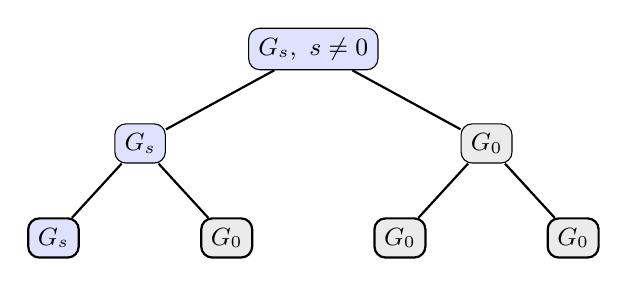
\begin{tikzpicture}[
  level distance=12mm,
  level 1/.style={sibling distance=44mm},
  level 2/.style={sibling distance=22mm},
  every node/.style={draw, rounded corners, inner sep=3.5pt, font=\small},
  edge from parent/.style={draw, thick}
]
\node[fill=blue!12] {$G_s,\ s \ne 0$}
  child {node[fill=blue!12] {$G_s$}
    child {node[fill=blue!12] {$G_s$}}
    child {node[fill=black!8] {$G_0$}}
  }
  child {node[fill=black!8] {$G_0$}
    child {node[fill=black!8] {$G_0$}}
    child {node[fill=black!8] {$G_0$}}
  };
\end{tikzpicture}
\caption{Two generations of lifts (\cref{prop:lift-symmetry}). A
shift-nonzero obstruction (blue) splits into one shift-nonzero and one
shift-zero child; a shift-zero obstruction (grey) splits into two shift-zero
children. Shift-zero is therefore \emph{absorbing} under lifting: it never
produces a shift-nonzero residue. The single persisting shift-nonzero line,
shedding one shift-zero child per level, is the combinatorial engine behind
the strict lift balance of \cref{cor:lift-balance}.}
\label{fig:lift-tree}
\end{figure}

% =============================================================================
\section{Positive density}
\label{sec:density}
% =============================================================================

\begin{proof}[Proof of \cref{thm:density-intro}]
By \cref{thm:lift-intro}, every $r_0 \in \Obs_{L_0}$ contributes two
distinct elements $r_0$ and $r_0 + 2^{L_0}$ to $\Obs_{L_0+1}$. Hence
$|\Obs_{L_0+1}| \ge 2 |\Obs_{L_0}|$, equivalently
$|\Obs_{L_0+1}|/2^{L_0+1} \ge |\Obs_{L_0}|/2^{L_0}$: the density ratio is
non-decreasing. Since $\Obs_L \subseteq \{1, \ldots, 2^L\}$ the ratio is
bounded above by $1$. By monotone convergence,
$c_W := \lim_{L \to \infty} |\Obs_L|/2^L$ exists in $[\rho_{L_0}, 1]$ for every
$L_0 \ge 5$. Two substitutions make this explicit:
\[
\begin{aligned}
|\Obs_{16}| = 7556 &\;\Rightarrow\; c_W \ge 7556/65536 \approx 0.115, \\
\Obs_6 = \{19, 27, 59\} &\;\Rightarrow\; c_W \ge 3/64,
\end{aligned}
\]
the first from the direct enumeration in Appendix~\ref{sec:appendix}
(Table~\ref{tab:appendix-counts}), the second the conservative bound at
$L_0 = 6$ (Section~\ref{sec:setup}). \qedhere
\end{proof}

The conservative bound $\rho_6 = 3/64$ uses only the three explicit
obstructions $\Obs_6 = \{19, 27, 59\}$. By raising $L_0$ and computing
$|\Obs_{L_0}|$ directly, tighter rigorous bounds for $c_W$ follow
(Table~\ref{tab:density-bounds}):

\begin{table}[ht]
\centering
\begin{tabular}{rrrr}
\toprule
$L_0$ & $|\Obs_{L_0}|$ & $\rho_{L_0}$ & rigorous lower bound for $c_W$ \\
\midrule
$6$  & $3$    & $\approx 0.047$ & $3/64$ \\
$10$ & $91$   & $\approx 0.089$ & $91/1024$ \\
$14$ & $1776$ & $\approx 0.108$ & $1776/16384$ \\
$16$ & $7556$ & $\approx 0.115$ & $7556/65536$ \\
$\vdots$ & $\vdots$ & $\vdots$ & $\vdots$ \\
$32$ & $631538769$ & $\approx 0.147$ & $631538769/2^{32}$ \\
\bottomrule
\end{tabular}
\caption{Rigorous lower bounds for $c_W$ obtained from finite-level enumeration of $\Obs_{L_0}$. The ratio $\rho_{L_0} := |\Obs_{L_0}|/2^{L_0}$ is non-decreasing in $L_0$ (\cref{thm:density-intro}).}
\label{tab:density-bounds}
\end{table}

These are not asymptotic estimates: they are finite-level computations
producing rigorous bounds at the cost of $O(L_0 \cdot 2^{L_0})$ operations
to enumerate obstructions modulo $2^{L_0}$. The exact value of $c_W$ is
not pinned down by this approach; we return to it in
Section~\ref{sec:Gs}.

% =============================================================================
\section{Full factor complexity}
\label{sec:fc}
% =============================================================================

\subsection{Setup}

To each $r \in \Obs_L$ we associate its binary representation as an
$L$-bit word, least significant bit first:
\[
w_r \in \{0,1\}^L, \qquad w_r[k] := \lfloor r / 2^k \rfloor \bmod 2, \quad k = 0, \ldots, L-1.
\]
In particular $w_r[0] = 1$ (since $r$ is odd) and $w_r[L-1]$ is the
leading bit of $r$ in this $L$-bit representation.
The \emph{language of obstruction words} at level $L$ is
$\Fac_L := \{w_r : r \in \Obs_L\}$, and the \emph{factor language} of the
obstruction family is
\[
\Fac(\Obs) := \{\, u \in \{0,1\}^* : u \text{ is a factor of } w_r \text{ for some } r \in \Obs_L,\, L \ge 5 \,\}.
\]
The \emph{factor complexity function} is
$p_W(\ell) := |\Fac(\Obs) \cap \{0,1\}^\ell|$. Trivially $p_W(\ell) \le 2^\ell$.

\subsection{The main theorem}

\begin{theorem*}[restating \cref{thm:fc-intro}]
For every $\ell \ge 0$, $p_W(\ell) = 2^\ell$.
\end{theorem*}

\begin{proof}
The case $\ell = 0$ is the empty word, which is trivially a factor of every
$w_r$, so $p_W(0) = 1 = 2^0$. Fix $\ell \ge 1$ and
$u = (u_0, u_1, \ldots, u_{\ell-1}) \in \{0,1\}^\ell$. Choose any anchor
$r_0 \in \Obs_6 = \{19, 27, 59\}$ (the set is confirmed by direct
enumeration; see Appendix~\ref{sec:appendix}). Define inductively
\[
r_k := r_{k-1} + u_{k-1} \cdot 2^{5 + k}, \qquad k = 1, 2, \ldots, \ell.
\]
We claim $r_k \in \Obs_{6+k}$ for each $k$. The base $k = 0$ is by choice of
$r_0$. For the inductive step from $k-1$ to $k$: if $u_{k-1} = 0$ then
$r_k = r_{k-1}$, so $r_k$ is the $r_+$ lift and lies in $\Obs_{6+k}$ by
\cref{thm:lift-plus}; if $u_{k-1} = 1$ then $r_k = r_{k-1} + 2^{5+k}$
is the $r_-$ lift and lies in $\Obs_{6+k}$ by \cref{thm:lift-minus}.

By construction,
\[
w_{r_\ell}[5+k] = u_{k-1} \qquad (k = 1, \ldots, \ell),
\]
so $u$ appears as a factor of $w_{r_\ell}$ occupying bit positions
$5+1, \ldots, 5+\ell$. Thus
$u \in \Fac(\Obs)$ for every $u \in \{0,1\}^\ell$, hence $p_W(\ell) \ge 2^\ell$.
Combined with the trivial upper bound, $p_W(\ell) = 2^\ell$. \qedhere
\end{proof}

In fact each of the three anchors in $\Obs_6$ individually realises every
pattern, as direct enumeration via the lift-symmetry table confirms; the
proof above needs only one.

\subsection{Entropy and substitution-shift rigidity}

The \emph{topological entropy} of a language $\mathcal{L} \subseteq \{0,1\}^*$
is $h(\mathcal{L}) := \limsup_{\ell \to \infty} (1/\ell) \log p_{\mathcal{L}}(\ell)$.
The factor-complexity function $p_{\mathcal{L}}$ itself goes back to the
foundational symbolic-dynamics papers of
Morse--Hedlund~\cite{MorseHedlund1938,MorseHedlund1940}. See
Lind--Marcus~\cite{LindMarcus1995} for general background on entropy of
subshifts and subshifts of finite type, Fogg~\cite{Fogg2002} or
Allouche--Shallit~\cite{AlloucheShallit2003} for factor complexity of
substitution and automatic sequences,
Cassaigne~\cite{Cassaigne1997} for the general theory of subword
complexity in terms of special factors, and
Berth\'e--Rigo~\cite{BertheRigo2010} and Lothaire~\cite{Lothaire2002}
for modern collected references on combinatorics on words, automata
and number theory.

\begin{corollary}\label{cor:entropy}
The topological entropy of $\Fac(\Obs)$ is $\log 2$.
\end{corollary}

This is the maximal value, matching that of the full Bernoulli shift
$\{0,1\}^\Z$.

\begin{corollary}
\label{cor:no-substitution}
The obstruction family $(\Obs_L)_{L \ge 5}$, viewed as a graded family of
finite languages over $\{0,1\}$, is
\begin{enumerate}[label=(\roman*)]
\item not the language of a proper subshift of finite type, that is, one
  defined by a non-empty list of forbidden factors;
\item not the language of a proper sofic shift in the classical sense
  (image of a proper SFT under a one-block factor map);
\item not the factor language of a primitive substitution shift in the
  sense of Pansiot~\cite{Pansiot1984} or Devyatov~\cite{Devyatov2015}.
\end{enumerate}
\end{corollary}

\begin{proof}
(i) A non-trivial SFT defined by a non-empty finite list of forbidden subwords
has entropy strictly less than $\log 2$ (Lind--Marcus~\cite{LindMarcus1995}),
contradicting \cref{cor:entropy}. (ii) A non-trivial sofic shift is the image of an
SFT under a one-block factor map and inherits the entropy constraint.
(iii) Primitive substitution shifts have factor complexity in one of the polynomial
classes $\Theta(1)$, $\Theta(n)$, $\Theta(n \log \log n)$, $\Theta(n \log n)$,
$\Theta(n^2)$ (Pansiot~\cite{Pansiot1984}; refined by
Devyatov~\cite{Devyatov2015}), and therefore have topological entropy
zero; the obstruction family has $p_W(\ell) = 2^\ell$ and hence entropy
$\log 2 > 0$, so it cannot be the factor language of a primitive
substitution shift. \qedhere
\end{proof}

\begin{remark}\label{rem:non-primitive}
The restriction to \emph{primitive} substitution shifts in
\cref{cor:no-substitution}(iii) is the scope of the
Pansiot--Devyatov classification we invoke. The entropy obstruction of
\cref{cor:entropy} in fact excludes the entire zero-entropy
regime, including all linearly recurrent subshifts, which contain the
primitive substitution shifts~\cite{DurandHostSkau1999}; the substitutive
candidates it does \emph{not} reach are therefore the non-primitive shifts
of positive entropy. Whether $\Fac(\Obs)$ can be realised as the factor
language of such a shift remains open (see Section~\ref{sec:open}). The same
question can be posed within the $S$-adic
framework~\cite{BertheDelecroix2014}, which builds sequences by composing
morphisms from a possibly infinite set and so reaches beyond single
primitive substitutions.
\end{remark}

% =============================================================================
\section{The \texorpdfstring{$G_s$}{Gs} classification}
\label{sec:Gs}
% =============================================================================

\subsection{Atomic obstructions}

An obstruction $r \in \Obs_L$ is \emph{atomic at level $L$} if
$r \bmod 2^{L-1} \notin \Obs_{L-1}$. We write $\Atom_L \subseteq \Obs_L$ and
$\Atom_L^{G_s} := \Atom_L \cap \Obs_L^{G_s}$.

\begin{lemma}[Atom decomposition]
\label{lem:atom-decomp}
For every $L \ge 5$,
\[
|\Obs_L| = \sum_{L_0 = 5}^{L} |\Atom_{L_0}| \cdot 2^{L - L_0}.
\]
\end{lemma}

\begin{proof}
We show that every $r \in \Obs_L$ has a unique smallest $L_0 \ge 5$ with
$r \bmod 2^{L_0} \in \Atom_{L_0}$. \emph{Existence:} starting from $r$ at
level $L$, consider the descending sequence $r_k := r \bmod 2^{L-k}$ for
$k = 0, 1, \ldots, L - 5$. By the lift theorem (\cref{thm:lift-intro}),
whenever $r_{k+1} \in \Obs_{L-k-1}$, the level-$(L-k)$ residue
$r_k = r \bmod 2^{L-k}$ is one of the two lifts of $r_{k+1}$ and hence
lies in $\Obs_{L-k}$; the converse need not hold. Let
$L_0$ be the smallest level $\ge 5$ for which
$r \bmod 2^{L_0} \in \Obs_{L_0}$. Then
$r \bmod 2^{L_0 - 1} \notin \Obs_{L_0 - 1}$: this holds by minimality of
$L_0$ when $L_0 > 5$, and because $\Obs_4 = \emptyset$
(\cref{rem:smallest-level}) when $L_0 = 5$. Hence
$r \bmod 2^{L_0} \in \Atom_{L_0}$.
\emph{Uniqueness:} the level $L_0$ is the smallest such by definition, hence
unique. Given the atomic anchor $r_0 := r \bmod 2^{L_0}$, the residue $r$ is
determined by $r_0$ together with the bits $\{u_{L_0}, \ldots, u_{L-1}\}$
encoding the lift choices (\cref{thm:lift-plus,thm:lift-minus}).
Each atomic anchor at level $L_0$ thus generates $2^{L - L_0}$ obstructions
at level $L$. \qedhere
\end{proof}

\subsection{No shift-zero atoms}

\begin{theorem}\label{thm:no-G0-atom}
For every $L \ge 7$, $|\Atom_L^{G_0}| = 0$.
\end{theorem}

The conclusion also holds at the base levels $L = 5, 6$ (see
\cref{cor:no-G0-atom-all}); the bound $L \ge 7$ in the statement
is conservative. At $L = 5$ it is vacuous, since $|\Obs_5^{G_0}| = 0$;
at $L = 6$ the unique shift-zero obstruction is $r = 27$, whose
reduction terminates at $J = 2$ with $\Vk^{(J)} = 5 = L - 1$, so it
would fall in Case~B below. We discharge both base cases formally by
direct enumeration in \cref{cor:no-G0-atom-all}.

\begin{proof}
Fix $L \ge 7$ and suppose $r \in \Obs_L^{G_0}$, so $\Xend(r, L) = 1$ with
shift index $s = 0$, i.e.\ $(c_J, d_J) = (1, 0)$. Write $r' := r \bmod 2^{L-1}$.
We first note $J \ge 2$: at $J = 0$ the terminal pair is $(2^{-v}, -2^{-v})$,
whose second coordinate $-2^{-v}$ is nonzero for every $v$, contradicting
$d_J = 0$; at $J = 1$ the update rule gives
\[
d_1 = \frac{3 \cdot (-2^{-v}) + 2^{-v} - 1}{2^{\vi^{(0)}}} = -\frac{1 + 2^{1-v}}{2^{\vi^{(0)}}},
\]
whose numerator is strictly negative for $v \ge 1$ (since $2^{1-v} + 1 > 0$),
so $d_1 \ne 0$, again contradicting $d_J = 0$. Hence $J \ge 2$, so the case
distinction below over the indices $J - 1$ and $J$ is well-defined.
The parallel reduction at $(r', L-1)$ starts from the same residue class
$a_K \bmod 2^{L-1}, a_I \bmod 2^{L-1-v}$ as at $(r, L)$, with the modulus
reduced by one power of two; the two K-tracks (resp.\ I-tracks) differ as
integers by $\Delta_K^{(j)} = 2^{L-1-\Vk^{(j)}} \cdot 3^j$ (resp.\
$\Delta_I^{(j)} = 2^{L-1-v-\Vi^{(j)}} \cdot 3^j$), in direct analogy with
the lift-minus calculation of \cref{thm:lift-minus}. Whenever
$\vk^{(j)} < L - 1 - \Vk^{(j)}$, the ultrametric identity forces
$v_2(3 a_K^{(j)} - 1)$ to agree at $(r, L)$ and $(r', L-1)$. Consequently the
per-step valuations $\vk^{(j)}, \vi^{(j)}$ and hence the affine data
$(c_j, d_j)$ coincide between the two reductions until the level-$(L-1)$
stop fires.

Termination of the reduction at $(r, L)$ at index $J$ means at least one
track satisfies its stop condition there; by \cref{cor:sync}, both
do. Since $s = 0$, at the terminal index $J$ the synchronisation
$\vi^{(J)} = \vk^{(J)} + 2s = \vk^{(J)}$ and
$\Vk^{(J)} - \Vi^{(J)} = v$ holds (\cref{lem:parity}). Hence the
K-track stop condition $\vk^{(J)} \ge L - \Vk^{(J)}$ and the I-track stop
condition $\vi^{(J)} \ge (L - v) - \Vi^{(J)}$ at $j = J$ are equivalent:
substituting $\Vi^{(J)} = \Vk^{(J)} - v$ and $\vi^{(J)} = \vk^{(J)}$
reduces the I-track condition to $\vk^{(J)} \ge L - \Vk^{(J)}$. Both
stop conditions at $j = J$ therefore read $\Vk^{(J)} + \vk^{(J)} \ge L$.
(The K- and I-track stop conditions are not in general equivalent at
$j < J$, so we rule out child stops on each track separately below;
the equivalence is used only at the terminal index $J$, where it
follows from $s = 0$.)
We split by the K-track value $\Vk^{(J)}$ (equivalently
$\Vk^{(J-1)} + \vk^{(J-1)}$): either $\Vk^{(J)} < L - 1$ (Case~A) or
$\Vk^{(J)} \ge L - 1$ (Case~B); these exhaust the integer possibilities.
We first rule out the level-$(L-1)$ stop on either track firing at any
earlier index $J' \le J - 2$. Suppose the K-track stop fired there, so
$\Vk^{(J')} + \vk^{(J')} \ge L - 1$. The $(r, L)$ reduction still takes its
$J'$-th step, since the level-$L$ stop has not yet fired at $J' < J$; this
gives $\Vk^{(J'+1)} \ge L - 1$, so the level-$L$ K-track modulus at index
$J'+1$ has valuation $L - \Vk^{(J'+1)} \le 1$. As $a_K^{(J'+1)}$ is odd,
$\vk^{(J'+1)} \ge 1$, so the next step is impossible and the $(r, L)$
reduction would stop at $J' + 1 \le J - 1$, contradicting the definition of
$J$. The same argument on the I-track, with $\Vi^{(J'+1)} \ge L - 1 - v$ and
oddness of $a_I^{(J'+1)}$, rules out a child I-stop at $J' \le J - 2$.
At index $J - 1$, a child I-stop requires $\Vi^{(J)} \ge L - 1 - v$;
by the terminal synchronisation $\Vi^{(J)} = \Vk^{(J)} - v$ (from
$s = 0$, equivalently $\delta_J = 0$), this is exactly
$\Vk^{(J)} \ge L - 1$ --- the Case~B branch below --- so in Case~A neither
child stop fires before index $J$.

\emph{Case A: $\Vk^{(J)} < L - 1$.} The K-track stop at level $L - 1$
does not fire at any index $\le J - 1$: the indices $J' \le J - 2$ are
ruled out by the preceding paragraph, and $J' = J - 1$ would
force $\Vk^{(J)} = \Vk^{(J-1)} + \vk^{(J-1)} \ge L - 1$, against
the Case-A hypothesis $\Vk^{(J)} < L - 1$. So the $(r', L-1)$ reduction
runs at least as far as index $J$; at $j = J$ we have
$\Vk^{(J)} + \vk^{(J)} \ge L > L - 1$, hence the K-track stop at level
$L - 1$ fires at $J$ and the reduction terminates there. (The I-track
stop at level $L - 1$ also fires at $J$ by the same chain, since at $j = J$
the synchronisation $\vi^{(J)} = \vk^{(J)}$, $\Vk^{(J)} - \Vi^{(J)} = v$
holds, but only the first track to stop matters for termination.) The
terminal data of the two reductions coincide: $(c_J, d_J) = (1, 0)$, so
$r' \in \Obs_{L-1}^{G_0}$ and $r$ is not atomic.

\emph{Case B: $\Vk^{(J)} \ge L - 1$, equivalently
$\Vk^{(J-1)} + \vk^{(J-1)} \ge L - 1$.} Combined with the standing
$\Vk^{(J-1)} + \vk^{(J-1)} < L$ (the level-$L$ stop does not fire
at $J - 1$), the only integer value is $\Vk^{(J)} = L - 1$. Hence the
K-track stop at level $L - 1$ fires at $J - 1$, and the $(r', L-1)$
reduction terminates one step earlier, at index $J - 1$, with terminal
data $(c_{J-1}, d_{J-1})$ (whether the I-track stop at level $L - 1$
also fires at $J - 1$ is immaterial for termination). From the update
rule (\cref{lem:affine}) at index $J - 1$,
\[
c_J = c_{J-1} \cdot 2^{\vk^{(J-1)} - \vi^{(J-1)}}, \qquad d_J = \frac{3 d_{J-1} + c_{J-1} - 1}{2^{\vi^{(J-1)}}}.
\]
Setting $c_J = 1$, $d_J = 0$ and reading off the numerator of $d_J$:
$3 d_{J-1} + c_{J-1} - 1 = 0$, i.e.\ $X_{J-1} = 1$. By the parity lemma
applied at the terminal index $J - 1$ of the reduction at $(r', L-1)$,
the terminal pair is in shift-$s'$ normal form for some $s' \in \Z$, so
$r' \in \Obs_{L-1}^{G_{s'}}$.

In either case, $r' \in \Obs_{L-1}$, so $r$ is not atomic. \qedhere
\end{proof}

\begin{corollary}\label{cor:no-G0-atom-all}
For every $L \ge 5$, $|\Atom_L^{G_0}| = 0$.
\end{corollary}

\begin{proof}
For $L \ge 7$, this is \cref{thm:no-G0-atom}. At the two base
levels direct enumeration (verified by \texttt{count\_obstructions.py})
gives $\Atom_5 = \{27\}$ and $\Atom_6 = \{19\}$, each with shift index
$s = 1 \ne 0$, so $|\Atom_5^{G_0}| = |\Atom_6^{G_0}| = 0$ as well.
\qedhere
\end{proof}

\subsection{Strict lift balance and series representation}

Write $g_L := |\Obs_L^{G_0}|$ and $h_L := |\Obs_L^{G_{\ne 0}}|$. The lift
symmetry of \cref{prop:lift-symmetry} gives, per parent at
$L - 1$ (Table~\ref{tab:lift-balance}):

\begin{table}[ht]
\centering
\begin{tabular}{c|cc}
\toprule
Parent at $L-1$ & Contribution to $g_L$ & Contribution to $h_L$ \\
\midrule
$G_0$ & $2$ & $0$ \\
$G_s$, $s \ne 0$ & $1$ & $1$ \\
\bottomrule
\end{tabular}
\caption{Per-parent contribution of a level-$(L-1)$ obstruction to the level-$L$ shift-zero and shift-nonzero populations under the two lifts $r_\pm$.}
\label{tab:lift-balance}
\end{table}

Summing and adding the atomic contributions, which by
\cref{cor:no-G0-atom-all} occur only in $h_L$:

\begin{corollary}[Strict lift balance]
\label{cor:lift-balance}
For every $L \ge 6$,
\[
g_L = 2 g_{L-1} + h_{L-1}, \qquad h_L = h_{L-1} + |\Atom_L^{G_{\ne 0}}|.
\]
Adding, $|\Obs_L| = 2 |\Obs_{L-1}| + |\Atom_L^{G_{\ne 0}}|$.
\end{corollary}

\begin{theorem}\label{thm:series}
The density constant $c_W$ admits the convergent series representation
\[
c_W = \frac{3}{64} + \sum_{L \ge 7} \frac{|\Atom_L^{G_{\ne 0}}|}{2^L},
\]
with non-negative terms. In particular, $|\Atom_L^{G_{\ne 0}}|/2^L \to 0$ as
$L \to \infty$.
\end{theorem}

\begin{proof}
By \cref{lem:atom-decomp} every $r \in \Obs_L$ has a unique atomic
anchor at some level $L_0 \in \{5, 6, \ldots, L\}$. By
\cref{cor:no-G0-atom-all}, $|\Atom_{L_0}^{G_0}| = 0$ for every
$L_0 \ge 5$, so each atom contributes to $\Atom_{L_0}^{G_{\ne 0}}$.
Direct enumeration at the two base levels (verified by
\texttt{count\_obstructions.py}) gives $\Atom_5 = \{27\}$ and
$\Atom_6 = \{19\}$, both with shift index $s = 1$, so
$|\Atom_5^{G_{\ne 0}}| = |\Atom_6^{G_{\ne 0}}| = 1$. Hence for every $L \ge 6$,
\[
|\Obs_L| = 2^{L-5} + 2^{L-6} + \sum_{L_0 = 7}^{L} |\Atom_{L_0}^{G_{\ne 0}}| \cdot 2^{L - L_0}
        = 3 \cdot 2^{L-6} + \sum_{L_0 = 7}^{L} |\Atom_{L_0}^{G_{\ne 0}}| \cdot 2^{L - L_0}.
\]
Dividing both sides by $2^L$,
\[
\rho_L = \frac{|\Obs_L|}{2^L} = \frac{3}{64} + \sum_{L_0 = 7}^{L} \frac{|\Atom_{L_0}^{G_{\ne 0}}|}{2^{L_0}}.
\]
By \cref{thm:density-intro}, $\rho_L$ is non-decreasing in $L$ and
bounded above by $1$, so its limit $c_W$ exists in $(0, 1]$. The
right-hand side is the $L$-th partial sum of a non-negative series with
fixed first term $3/64$; since the partial sums converge to $c_W$, the
series converges, with sum $c_W$ and tail $|\Atom_L^{G_{\ne 0}}|/2^L \to 0$
as $L \to \infty$. \qedhere
\end{proof}

\subsection{The shift-index window}
\label{sec:shift-window}

The $G_s$ classification raises the question of which shift classes can be
nonempty at a given level. We show that the \emph{nontrivial} classes
($|s| \ge 2$) occupy only a window of shift indices of width $O(L)$. The engine
is a lower bound on the termination index $J$ in terms of $|s|$: an obstruction
of large shift index reduces slowly. The bound is sharp --- for instance
$r = 15877 \in \Obs_{15}^{G_2}$ terminates at $J = 7 = 2\cdot 2 + 3$ with terminal
data $(c_J, d_J) = (16, -5) = \bigl(4^2, (1-4^2)/3\bigr)$, and
$r = 1015979 \in \Obs_{21}^{G_{-2}}$ likewise has $J = 7$. We emphasise at the
outset what the resulting window does \emph{not} give: it bounds the
\emph{number} of nonempty shift classes per level, not their populations, and so
does not by itself resolve the growth question of Section~\ref{sec:cW-open}
(\cref{rem:window-scope}).

Throughout this subsection $s = s(r, L)$ is the (signed) shift index of an
obstruction $r \in \Obs_L$, $J = J(r, L)$ its termination index, $v = \vtwo(r-1)$,
and we set $q := \Vi^{(J)} - J$. Since the I-track takes $J$ steps, each of
valuation $\ge 1$ (as $3 a_I^{(j)} - 1$ is even for odd $a_I^{(j)}$),
$\Vi^{(J)} \ge J$, so $q \ge 0$.

\begin{lemma}[K-track prefix]\label{lem:k-prefix}
For every odd $r > 1$ with $v = \vtwo(r-1)$, the K-track of the parallel reduction
satisfies $\vk^{(j)} = 1$ for $0 \le j \le v-2$ and $\vk^{(v-1)} \ge 2$. Hence
$\Vk^{(j)} = j$ for $0 \le j \le \min(v-1, J)$.
\end{lemma}

\begin{proof}
Write $r = 1 + 2^v m$ with $m$ odd. We claim $a_K^{(j)} = 1 + 3^{\,j} 2^{\,v-j} m$
for $0 \le j \le v-1$. The base case $j = 0$ is the definition. If it holds at
$j \le v-2$, then
$3 a_K^{(j)} - 1 = 2 + 3^{\,j+1} 2^{\,v-j} m = 2\bigl(1 + 3^{\,j+1} 2^{\,v-j-1} m\bigr)$,
and $1 + 3^{\,j+1} 2^{\,v-j-1} m$ is odd because $v-j-1 \ge 1$; thus
$\vk^{(j)} = 1$ and $a_K^{(j+1)} = 1 + 3^{\,j+1} 2^{\,v-(j+1)} m$, completing the
induction. At $j = v-1$,
$3 a_K^{(v-1)} - 1 = 2 + 3^{\,v} 2 m = 2\bigl(1 + 3^{\,v} m\bigr)$ with
$1 + 3^{\,v} m$ even (both $3^v$ and $m$ are odd), so $\vk^{(v-1)} \ge 2$. The
cumulative statement follows by summing the unit valuations. (For $v = 1$ the
first claim is vacuous and the second reads $\vk^{(0)} \ge 2$.)
\qedhere
\end{proof}

\begin{lemma}[Minimal depth]\label{lem:depth-min}
Every obstruction with shift index $s \ge 0$ has $J \ge v$.
\end{lemma}

\begin{proof}
If $J \le v-1$, then $\Vk^{(J)} = J$ by \cref{lem:k-prefix}. But
$\Vk^{(J)} = \Vi^{(J)} + 2s + v \ge J + 2s + v \ge J + v$, forcing $v \le 0$, a
contradiction.
\qedhere
\end{proof}

\begin{lemma}[Sign-free obstruction identity]\label{lem:signfree}
For every $r \in \Obs_L$, with cumulative valuations along the two tracks and
termination index $J$,
\begin{equation}\label{eq:signfree}
\sum_{j=0}^{J} 3^{\,J-j} 2^{\Vk^{(j)}}
   \;=\; 3^{\,J+1} \;+\; 2^{v} \sum_{j=0}^{J} 3^{\,J-j} 2^{\Vi^{(j)}}.
\end{equation}
The sign of $s$ does not enter; equivalently, with the terminal terms removed,
\begin{equation}\label{eq:oform}
\sum_{j=0}^{J-1} 3^{\,J-j}\bigl(2^{\Vk^{(j)}} - 2^{\Vi^{(j)}+v}\bigr)
   \;=\; 3^{\,J+1} + 2^{\Vi^{(J)}+v}\bigl(1 - 4^{s}\bigr).
\end{equation}
\end{lemma}

\begin{proof}
Set $\tilde n_j := 2^{\Vi^{(j)}+v} d_j$. Iterating
$c_{j+1} = c_j 2^{\vk^{(j)} - \vi^{(j)}}$ from $c_0 = 2^{-v}$ (\cref{lem:affine})
gives $c_j = 2^{\Vk^{(j)} - \Vi^{(j)} - v}$, so $2^{\Vi^{(j)}+v} c_j = 2^{\Vk^{(j)}}$.
The update $d_{j+1} = (3 d_j + c_j - 1)/2^{\vi^{(j)}}$ then yields
\[
\tilde n_{j+1} = 2^{\Vi^{(j)}+v}\bigl(3 d_j + c_j - 1\bigr)
   = 3\,\tilde n_j + 2^{\Vk^{(j)}} - 2^{\Vi^{(j)}+v},
\qquad \tilde n_0 = 2^{v} d_0 = -1 .
\]
Unrolling and multiplying by $3$, using
$3 \tilde n_J = 2^{\Vi^{(J)}+v} \cdot 3 d_J = 2^{\Vi^{(J)}+v}(1 - 4^{s})$ from the
shift-$s$ normal form, gives~\eqref{eq:oform}. Since
$\Vk^{(J)} = \Vi^{(J)} + v + 2s$, the right-hand side of~\eqref{eq:oform} equals
$3^{J+1} + 2^{\Vi^{(J)}+v} - 2^{\Vk^{(J)}}$; moving the two terminal terms into the
respective sums turns~\eqref{eq:oform} into~\eqref{eq:signfree}.
\qedhere
\end{proof}

The bound itself splits by the size and sign of $s$. The two large-shift regimes
are analytic; the small-shift tails are finite computations.

\begin{lemma}[Large negative shift]\label{lem:depth-negbig}
Every obstruction with $s \le -4$ has $J \ge 2|s| + 3$.
\end{lemma}

\begin{proof}
Write $a = |s|$ and abbreviate
\[
\hat A_K = \sum_{j=0}^{J} 3^{J-j} 2^{\Vk^{(j)}}, \qquad
\hat A_I = \sum_{j=0}^{J} 3^{J-j} 2^{\Vi^{(j)}},
\]
so \eqref{eq:signfree} reads $\hat A_K = 3^{J+1} + 2^{v} \hat A_I$. We use two
elementary bounds. Keeping only the $j = J$ term of $\hat A_I$ (all terms
positive) and using $\Vi^{(J)} + v = \Vk^{(J)} + 2a$,
\[
2^{v} \hat A_I \;\ge\; 2^{\Vi^{(J)}+v} \;=\; 2^{\Vk^{(J)} + 2a}.
\]
Since the valuations increase by at least $1$ per step, $\Vk^{(j)} \le \Vk^{(J)} - (J-j)$, whence
\[
\hat A_K \;\le\; 2^{\Vk^{(J)}} \sum_{i=0}^{J} (3/2)^{i}
   \;<\; 2^{\Vk^{(J)}} \cdot \frac{3^{J+1}}{2^{J}} .
\]
As $\hat A_K > 2^{v}\hat A_I$, combining gives $2^{\Vk^{(J)}+2a} < 2^{\Vk^{(J)}} 3^{J+1}/2^{J}$, i.e.
\begin{equation}\label{eq:Nbound}
3^{\,J+1} > 2^{\,J + 2a}. \tag{N}
\end{equation}
The ratio $f(J) := 3^{J+1}/2^{J+2a}$ is strictly increasing, and
\[
f(2a+2) = \frac{3^{\,2a+3}}{2^{\,4a+2}} = \frac{27}{4}\Bigl(\frac{9}{16}\Bigr)^{a} < 1
\iff a \ge 4 .
\]
Hence for $a \ge 4$ every $J \le 2a+2$ violates~\eqref{eq:Nbound}, so $J \ge 2a+3$.
\qedhere
\end{proof}

\begin{lemma}[Large positive shift]\label{lem:depth-posbig}
Every obstruction with $s \ge 4$ has $J \ge 2s + 3$.
\end{lemma}

\begin{proof}
By \cref{lem:depth-min}, $v \le J$. Write the O''-form~\eqref{eq:oform} as
$A_K - 2^{v} A_I = 3^{J+1} + 2^{\,J+q+v}(1 - 4^{s})$ with
$A_K = \sum_{j=0}^{J-1} 3^{J-j} 2^{\Vk^{(j)}}$ and $A_I$ analogous, using
$\Vi^{(J)} = J + q$. The two sums range over the structural families: by
\cref{lem:k-prefix} the K-valuations satisfy $\Vk^{(j)} = j$ for $j \le v-1$,
$\Vk^{(j)} \ge j+1$ for $v \le j \le J-1$; the I-valuations satisfy
$\Vi^{(0)} = 0$, $\Vi^{(j+1)} > \Vi^{(j)}$, $\Vi^{(J)} = J+q$. Minimising $A_K$ and
maximising $A_I$ over these families \emph{independently} can only decrease
$A_K - 2^{v} A_I$, so the decoupled deficit
\[
D := (A_K^{\min} - 2^{v} A_I^{\max}) - \bigl(3^{J+1} + 2^{J+q+v}(1-4^{s})\bigr)
\]
satisfies $D > 0 \Rightarrow$ no obstruction with these parameters. Both optima
are attained by saturating the structural bounds just listed: since the common
weight $3^{J-j}$ in $A_K$ and $A_I$ decreases strictly in $j$, each sum is
extremised at the envelope of its constraints. Concretely, $A_I^{\max}$ takes
the I-valuations as large as the endpoint $\Vi^{(J)} = J+q$ and strict
monotonicity allow, putting all I-excess in the first step; $A_K^{\min}$ keeps
the K-valuations on their lower envelope, with the single forced jump of
\cref{lem:k-prefix} deferred to the final, uncounted step. Both extremal sums
are independently confirmed by a brute optimisation over the families in
Appendix~\ref{sec:appendix}. This gives the closed forms
\[
A_I^{\max} = 3^{J} + 2^{q}\bigl(2\cdot 3^{J} - 3\cdot 2^{J}\bigr),
\qquad
A_K^{\min} = 3^{J+1} + 2^{v} 3^{\,J-v+1} - 6\cdot 2^{J},
\]
and, after the $3^{J+1}$ cancels,
\[
D = C_0(J,v) + 2^{\,v+q}\,\Gamma(J,s),
\]
where $\Gamma(J,s) = 2^{J}(4^{s}+2) - 2\cdot 3^{J}$ and
$C_0(J,v) = 2^{v} 3^{J}\bigl(3^{1-v}-1\bigr) - 6\cdot 2^{J}$. Here $\Gamma$
governs the $q$-dependence of $D$ and $C_0$ the $q$-independent $(J,v)$-terms;
the $q=0$ specialisation below splits $D$ further into a $q=0$ envelope $\Phi$
and a $v$-correction $R$.
For $s \ge 3$ and $1 \le J \le 2s+2$ one has $\Gamma(J,s) > 0$: the sign change
$2^{J}(4^{s}+2) = 2\cdot 3^{J}$ occurs at $J \approx s\log_{3/2}4 > 2s+2$. Hence $D$ is
non-decreasing in $q$ and $q = 0$ is the worst case. At $q = 0$,
$D(J,s,v,0) = 2^{v}\,\Phi(J,s) + R(J,v)$, where
$\Phi(J,s) = 2^{J}(4^{s}+2) - 3^{J+1}$ and
$R(J,v) = 2^{v} 3^{\,J-v+1} - 6\cdot 2^{J}$.
For $s \ge 4$ and $J \le 2s+2$, $\Phi(J,s) > 3$ (worst case $J = 2s+2$:
$\Phi(2s+2,s) > 3 \iff (16/9)^{s} > 27/4$, which holds for $s \ge 4$). Finally
$R(J,v) = 3\cdot 2^{v}\bigl(3^{\,J-v} - 2^{\,J-v+1}\bigr)$ is $\ge 0$ when
$J - v \ge 2$ and equals $-3\cdot 2^{v}$ when $J - v \in \{0,1\}$; in the first
case $D(J,s,v,0) \ge 2^{v}\Phi > 0$, in the second
$D(J,s,v,0) = 2^{v}(\Phi - 3) > 0$. Thus $D > 0$ for all $q \ge 0$ and all
$1 \le v \le J \le 2s+2$, so no obstruction has $J \le 2s+2$.
\qedhere
\end{proof}

The remaining strata are the small shifts $|s| \in \{2,3\}$. After the analytic
bounds only finitely many configurations survive, and they are settled by an
exact finite computation. The key device is a bounded carry automaton, which
decides a whole stratum for \emph{all} $q$ at once.

\begin{lemma}[Bounded carry automaton]\label{lem:carry-automaton}
Fix a stratum $(s, J)$ and $v$. Reading the integer
identity~\eqref{eq:signfree} bit position by bit position defines a finite
automaton whose state is $(\text{carry}, \#\{\Vk\text{ placed}\}, \#\{\Vi\text{ placed}\})$.
Each strictly increasing valuation contributes one set bit, and the carry is
bounded, each transition halving it towards a fixed invariant interval. An
obstruction with parameter $q$ then corresponds exactly to an accepting run
(carry $0$, all valuations placed). The positions factor as $\text{prefix} \to \text{block } A
\to \text{block } B \to \text{tail}$, where block $A$ carries a single
$q$- and position-independent transition $T_A$ whose \emph{length} is the only
$q$-dependence, block $B$ has fixed width $2|s|+1$, and the tail accepts iff the
incoming carry is $0$ (Figure~\ref{fig:carry-blocks}). Since the state space is
finite, the reachable-set sequence $R_m = T_A^{\,m}(R_0)$ is eventually periodic;
acceptance therefore depends on $q$ only through $R_{\,m(q)}$ and is periodic in
$q$ past a preperiod. A finite check over one preperiod plus one period decides
the stratum for every $q \ge 0$.
\end{lemma}

\begin{figure}[ht]
\centering
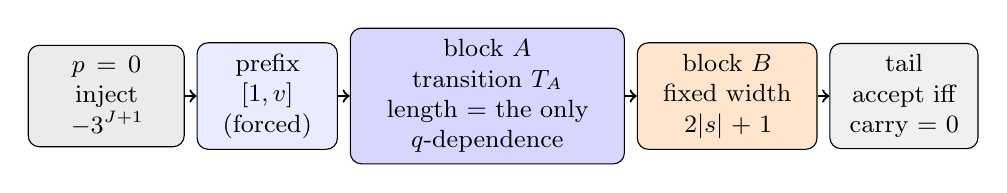
\begin{tikzpicture}[
  every node/.style={font=\small},
  box/.style={draw, rounded corners, minimum height=11mm, inner sep=4pt, align=center}
]
\node[box, fill=black!8, text width=17mm] (inj) {$p = 0$\\inject\\$-3^{J+1}$};
\node[box, fill=blue!8, text width=15mm, right=1.5mm of inj] (pre) {prefix\\$[1,v]$\\(forced)};
\node[box, fill=blue!16, text width=32mm, right=1.5mm of pre] (A) {block $A$\\transition $T_A$\\length $=$ the only\\$q$-dependence};
\node[box, fill=orange!20, text width=20mm, right=1.5mm of A] (B) {block $B$\\fixed width\\$2|s|+1$};
\node[box, fill=black!6, text width=16mm, right=1.5mm of B] (tail) {tail\\accept iff\\carry $= 0$};
\draw[->, thick] (inj) -- (pre);
\draw[->, thick] (pre) -- (A);
\draw[->, thick] (A) -- (B);
\draw[->, thick] (B) -- (tail);
\end{tikzpicture}
\caption{Block factorisation of the carry automaton of
\cref{lem:carry-automaton}. Only the \emph{length} of block $A$ depends on $q$;
the transition $T_A$ does not. As $T_A^{\,m}(R_0)$ is eventually periodic, a
finite computation over one preperiod and one period decides the stratum for all
$q$. The fixed-point data (preperiods, periods, reachable-state counts) per
stratum are tabulated in Appendix~\ref{sec:appendix}.}
\label{fig:carry-blocks}
\end{figure}

\begin{lemma}[Small-shift tails]\label{lem:finite-tails}
No obstruction has $|s| \in \{2,3\}$ and $J \le 2|s| + 2$.
\end{lemma}

\begin{proof}
For $s \le -2$ the inequality~\eqref{eq:Nbound} (which used only
$|s| \ge 2$) rules out every $J \le 2|s|+2$ except the strata
$(|s|, J) \in \{(2,5), (2,6), (3,8)\}$; each is closed for all $q$ by
\cref{lem:carry-automaton}. For $s \ge 2$ the decoupled deficit $D$ of
\cref{lem:depth-posbig} is positive except on a finite, explicitly enumerated
set: for $s = 3$ only the cells $(J=8,\, q=0,\, v \in \{2,\dots,8\})$ survive,
and for $s = 2$ only $(J=5,\, q \in \{0,1\})$ together with the single stratum
$J = 6$. The stratum $(s=2, J=6)$ is special: there $\Gamma(6,2) < 0$ leaves
$q$ unbounded, and it is closed for all $q$ by \cref{lem:carry-automaton}. The
finitely many residual cells are closed by exhaustive search over the coupled
valuation sequences. All
these checks are reproducible and are recorded in Appendix~\ref{sec:appendix}.
\qedhere
\end{proof}

\begin{theorem}[Depth bound]\label{thm:depth}
Every obstruction with $|s| \ge 2$ satisfies $J \ge 2|s| + 3$.
\end{theorem}

\begin{proof}
For $s \ge 4$ this is \cref{lem:depth-posbig}; for $s \le -4$,
\cref{lem:depth-negbig}; for $|s| \in \{2,3\}$, \cref{lem:finite-tails} rules out
$J \le 2|s|+2$.
\qedhere
\end{proof}

\begin{corollary}[Shift-index window]\label{cor:shift-window}
Let $r \in \Obs_L$ with $v = \vtwo(r-1)$. If $s \ge 2$, then
\[
s \le \frac{L - 4 - v}{4} \le \Bigl\lfloor \tfrac{L-5}{4} \Bigr\rfloor ;
\]
if $s \le -2$, then $s \ge -\dfrac{L-4-v}{2}$. In particular at most $O(L)$ of the
classes $\Obs_L^{G_s}$ are nonempty.
\end{corollary}

\begin{proof}
For $s \ge 2$, \cref{thm:depth} gives $J \ge 2s+3$, and
$\Vk^{(J)} = \Vi^{(J)} + 2s + v \ge J + 2s + v \ge 4s + 3 + v$; with
$\Vk^{(J)} \le L-1$ (\cref{lem:parity}) this yields $4s + 3 + v \le L-1$, i.e.
$s \le (L-4-v)/4 \le (L-5)/4$ as $v \ge 1$. For $s \le -2$, $\Vi^{(J)} \ge J \ge 2|s|+3$
and $\Vi^{(J)} \le L-1-v$ (\cref{lem:parity}) give $2|s|+3 \le L-1-v$, i.e.
$s \ge -(L-4-v)/2$. The shift indices of the nontrivial classes thus lie in an
interval of length $O(L)$; the three classes $|s| \le 1$ add a constant.
\qedhere
\end{proof}

The window is asymmetric: the positive side scales like $L/4$, the negative side
like $L/2$. The asymmetry is structural --- on the positive side
$\Vk^{(J)} = \Vi^{(J)} + 2s + v$ contributes the extra $2s$ gap that yields the
factor $4$, whereas on the negative side the high-ending track is the I-track and
only the factor $2$ survives. The depth bound $J \ge 2|s| + 3$ of
\cref{thm:depth}, by contrast, is fully two-sided.

\begin{remark}\label{rem:window-scope}
\cref{cor:shift-window} bounds the \emph{number} of nonempty shift classes at
level $L$ by $O(L)$, hence the support of the shift distribution is a window of
width $O(L)$. It does not bound the \emph{population} $|\Obs_L^{G_s}|$ of any
class, and in particular gives no bound on $|\Atom_L^{G_{\ne 0}}|$; it therefore
does not resolve the growth question of $c_W$ taken up in
Section~\ref{sec:cW-open}.
\end{remark}

\subsection{The remaining open question}

\cref{thm:series} reduces the question of $c_W$'s exact value to
controlling the growth of $|\Atom_L^{G_{\ne 0}}|$. A bound of the form
$|\Atom_L^{G_{\ne 0}}| \le C \cdot \alpha^L$ with $\alpha < 2$ would give a
geometrically convergent series with explicit error bounds. We do not
establish such a bound here; we return to the question in
Section~\ref{sec:open}.

% =============================================================================
\section{The \texorpdfstring{$T_+$}{T+} side}
\label{sec:tplus}
% =============================================================================

The classical Collatz map $\Tplus$ admits the same obstruction theory.
We transfer the framework of Section~\ref{sec:setup} to $\Tplus$ and
show that the residue involution $r \mapsto \overline{r} := 2^L - r$
realises an explicit bijection between the two obstruction families,
step-by-step at the level of the parallel reduction.

\subsection{The \texorpdfstring{$\Tplus$}{T+} parallel reduction}

Fix a positive odd integer $r$ with $\vtwo(r+1) \ge 1$, and write
$v := \vtwo(r+1)$ and $m := (r+1)/2^v$; then $m$ is odd. For a level
$L > v$, run the parallel reduction with $\Tplus$:
\begin{itemize}
\item the \emph{K-track}, starting from $(a_K^{(0)}, b_K^{(0)}) := (r, 2^L)$
  with basic step $a_K' = (3 a_K + 1)/2^{\vk}$,
  $\vk := \vtwo(3 a_K + 1)$;
\item the \emph{I-track}, starting from
  $(a_I^{(0)}, b_I^{(0)}) := (m, 2^{L - v})$ with the analogous basic step.
\end{itemize}
The initial relation $m = (r+1)/2^v$ writes as
$a_I^{(0)} = 2^{-v} a_K^{(0)} + 2^{-v}$, so the affine relation
$a_I^{(j)} = c_j a_K^{(j)} + d_j$ holds at index~$0$ with
$c_0 = 2^{-v}$, $d_0 = +2^{-v}$. The derivation of
\cref{lem:affine}, applied with $\Tplus$ in place of $\Tminus$ and
using $3 a_I + 1 = c_j (3 a_K + 1) + (3 d_j - c_j + 1)$, yields the
update rule
\[
c_{j+1} = c_j \cdot 2^{\vk^{(j)} - \vi^{(j)}}, \qquad
d_{j+1} = \frac{3 d_j - c_j + 1}{2^{\vi^{(j)}}}.
\]
(The numerator changes sign relative to the $\Tminus$ rule.) We define
the $\Tplus$-analogue of the $X$-invariant by
\[
\Xend^{+}(r, L) := c_J - 3 d_J,
\]
where $J$ is the termination index. An odd $r$ with $\vtwo(r+1) \ge 1$
and $L > \vtwo(r+1)$ is a \emph{$\Tplus$-obstruction residue at level $L$}
if $\Xend^{+}(r, L) = 1$; we write $\Obs_L^{+} \subseteq \{1, \ldots, 2^L\}$
for the set of such residues.

\begin{remark}\label{rem:Xplus-sign}
The sign convention $\Xend^{+} := c - 3d$ (rather than $3d + c$) is the
one forced by the affine algebra: with this combination the analogue of
the parity lemma (\cref{lem:parity}) yields the shift-$s$ normal
form $(c_J, d_J) = (4^s, (4^s - 1)/3)$, and the residue-level bijection
of \cref{thm:tplus-bijection} below is exact.
\end{remark}

\subsection{The residue involution}

\begin{lemma}[Residue-level involution]\label{lem:involution-step}
Let $r$ be odd with $v := \vtwo(r-1) \ge 1$ and $L > v$, and set
$\overline{r} := 2^L - r$; here $r$ is the $\Tminus$ residue and
$\overline{r}$ its $\Tplus$ partner. In the conclusions below, write
$\Vk^{(j)} := \sum_{i < j} \vk^{(i)}$ and
$\Vi^{(j)} := \sum_{i < j} \vi^{(i)}$ for the cumulative valuations
along the two tracks; the proof shows that they coincide across the
$\Tplus$ and $\Tminus$ reductions, so a single notation suffices.
Conclusions:
\begin{enumerate}[label=(\roman*)]
\item $\overline{r}$ is odd with $\vtwo(\overline{r} + 1) = v < L$
  (so the $\Tplus$ reduction at $\overline{r}$ in the sense of
  Section~\ref{sec:tplus} uses the same parameter $v$);
\item the $\Tminus$ parallel reduction at $(r, L)$ and the $\Tplus$
  parallel reduction at $(\overline{r}, L)$, both with parameter $v$,
  terminate at the same index $J$;
\item for every $0 \le j \le J$,
\begin{equation}\label{eq:invol-residue}
a_K^{+,(j)} \equiv -\, a_K^{-,(j)} \pmod{2^{L - \Vk^{(j)}}},
\quad
a_I^{+,(j)} \equiv -\, a_I^{-,(j)} \pmod{2^{L - v - \Vi^{(j)}}},
\end{equation}
and $\vk^{+,(j)} = \vk^{-,(j)}$, $\vi^{+,(j)} = \vi^{-,(j)}$
whenever $j < J$;
\item the affine data satisfy
\begin{equation}\label{eq:invol-affine}
(c_j^{+}, d_j^{+}) = (c_j^{-},\; -\, d_j^{-}) \qquad (0 \le j \le J).
\end{equation}
\end{enumerate}
\end{lemma}

\begin{proof}
(i): $\overline{r} + 1 = 2^L - (r - 1)$ has, by the ultrametric identity
with $\vtwo(r-1) = v < L$, $2$-adic valuation exactly $v$. Oddness of
$\overline{r}$ is immediate.

(iii) and (ii) jointly: we prove the residue congruences
in~\eqref{eq:invol-residue} for $j = 0, 1, \ldots$ by induction, and
deduce simultaneous termination and the valuation equalities along the
way.

\emph{Base case ($j = 0$).} K-track:
$a_K^{+,(0)} = \overline{r} = 2^L - r = -a_K^{-,(0)} + 2^L$.
I-track: $a_I^{-,(0)} = (r-1)/2^v$ and
$a_I^{+,(0)} = (\overline{r}+1)/2^v = (2^L - (r-1))/2^v = 2^{L-v} - a_I^{-,(0)}$.
Both congruences in~\eqref{eq:invol-residue} hold at $j = 0$. For the
valuation equality at $j = 0$, suppose the $\Tminus$ reduction is still
running, i.e.\ $\vk^{-,(0)} < L$. Then
$3 \overline{r} + 1 = 3 \cdot 2^L - (3 r - 1)$ has summands of
valuations $L$ and $\vk^{-,(0)}$ respectively, with $\vk^{-,(0)} < L$;
the ultrametric identity gives $\vk^{+,(0)} = \vk^{-,(0)}$. The
analogous calculation on the I-track gives $\vi^{+,(0)} = \vi^{-,(0)}$.

\emph{Inductive step.} Assume~\eqref{eq:invol-residue} at index $j$ and
that both reductions are still running at index $j$ --- so
$\vk^{(j)} < L - \Vk^{(j)}$ and $\vi^{(j)} < L - v - \Vi^{(j)}$, with the
valuations equal across $+/-$ by the inductive valuation equalities. For the
K-track,
\[
3 a_K^{+,(j)} + 1 \equiv 3 (-a_K^{-,(j)}) + 1 = -(3 a_K^{-,(j)} - 1)
\pmod{2^{L - \Vk^{(j)}}}.
\]
The right-hand side has valuation $\vk^{(j)} < L - \Vk^{(j)}$, so the
left-hand side has the same valuation $\vk^{+,(j)} = \vk^{(j)}$, and
dividing through by $2^{\vk^{(j)}}$ gives
\[
a_K^{+,(j+1)} = \frac{3 a_K^{+,(j)} + 1}{2^{\vk^{(j)}}}
\equiv -\, \frac{3 a_K^{-,(j)} - 1}{2^{\vk^{(j)}}}
= -\, a_K^{-,(j+1)}
\pmod{2^{L - \Vk^{(j+1)}}}.
\]
The same calculation on the I-track --- replacing $L - \Vk$ by
$L - v - \Vi$ and $3a-1$ by the I-track numerator --- gives the analogous
congruence and $\vi^{+,(j)} = \vi^{(j)}$.

\emph{Simultaneous termination.} The termination condition of the
$(\overline{r}, L)$ reduction at index $j$ is
$\vk^{+,(j)} \ge L - \Vk^{(j)}$ or $\vi^{+,(j)} \ge L - v - \Vi^{(j)}$.
We show termination at exactly $J$ in two directions. \emph{No earlier
stop:} if the $\Tplus$ reduction stopped at some $j' < J$, then by the
inductive step at $j'$ (valid because both reductions still run at $j'$)
the valuation equalities $\vk^{+,(j')} = \vk^{-,(j')}$ and
$\vi^{+,(j')} = \vi^{-,(j')}$ hold, so the $\Tminus$ reduction would
also satisfy its stop condition at $j'$, contradicting the definition
of $J$. \emph{Stop at $J$:} the residue congruence~\eqref{eq:invol-residue}
at $j = J$ follows by applying the inductive step one final time, valid
because the inductive hypothesis at $j = J - 1$ only requires the reductions
to be running there, not at $J$. Combining this congruence with the
$\Tminus$ K-track stop
$3 a_K^{-,(J)} - 1 \equiv 0 \pmod{2^{L - \Vk^{(J)}}}$ yields
\[
3 a_K^{+,(J)} + 1 \equiv -(3 a_K^{-,(J)} - 1) \equiv 0 \pmod{2^{L - \Vk^{(J)}}},
\]
so $\vk^{+,(J)} \ge L - \Vk^{(J)}$ and the $\Tplus$ K-track stops at $J$; the
analogous calculation on the I-track gives
$\vi^{+,(J)} \ge L - v - \Vi^{(J)}$.

(iv): At $j = 0$, $c_0^{+} = 2^{-v} = c_0^{-}$ and
$d_0^{+} = +2^{-v} = -\, d_0^{-}$. Inductively, given
$(c_j^{+}, d_j^{+}) = (c_j^{-}, -d_j^{-})$ and the valuation equalities
$\vk^{+,(j)} = \vk^{-,(j)}$, $\vi^{+,(j)} = \vi^{-,(j)}$,
\begin{align*}
c_{j+1}^{+} &= c_j^{+} \cdot 2^{\vk^{(j)} - \vi^{(j)}} = c_{j+1}^{-}, \\
d_{j+1}^{+} &= \frac{3 d_j^{+} - c_j^{+} + 1}{2^{\vi^{(j)}}}
  = -\,\frac{3 d_j^{-} + c_j^{-} - 1}{2^{\vi^{(j)}}}
  = -\, d_{j+1}^{-}. \qedhere
\end{align*}
\end{proof}

\subsection{The bijection theorem}

\begin{theorem}\label{thm:tplus-bijection}
For every level $L$, the involution $r \mapsto \overline{r} := 2^L - r$
restricts to a bijection $\Obs_L \leftrightarrow \Obs_L^{+}$.
Consequently $|\Obs_L^{+}| = |\Obs_L|$, and
\cref{thm:lift-intro,thm:density-intro,thm:fc-intro}
hold verbatim for $\Obs^{+}$, with the same density constant $c_W$ and
factor complexity function $p_W^{+}(\ell) = 2^\ell$.
\end{theorem}

\begin{proof}
For $r$ odd with $\vtwo(r-1) \ge 1$ and $L > \vtwo(r-1)$, equation
\eqref{eq:invol-affine} of \cref{lem:involution-step}(iv) at the
terminal index $J$ together with the sign convention
$\Xend^{+} := c - 3d$ of \cref{rem:Xplus-sign} gives
\[
\Xend^{+}(\overline{r}, L) = c_J^{+} - 3 d_J^{+}
  = c_J^{-} - 3 \cdot (-d_J^{-})
  = c_J^{-} + 3 d_J^{-}
  = \Xend(r, L).
\]
Hence $r \in \Obs_L$ iff $\overline{r} \in \Obs_L^{+}$. Since
$r \mapsto \overline{r}$ is an involution on the odd residues in
$\{1, \ldots, 2^L - 1\}$, it restricts to a bijection
$\Obs_L \leftrightarrow \Obs_L^{+}$. Concretely, at $L = 5$ this gives
$\Obs_5^{+} = \{5\}$, and at $L = 6$ it gives
$\Obs_6^{+} = \{2^6 - r : r \in \Obs_6\} = \{5, 37, 45\}$, the anchor set
parallel to $\Obs_6$ in the $\Tplus$ analogue of the
factor-complexity construction below.

For the remaining claims, observe that
\cref{lem:involution-step} conjugates each $\Tminus$ basic step
into the corresponding $\Tplus$ basic step.

\emph{Lift.} The $\Tplus$ lift theorem (the analogue of
\cref{thm:lift-intro}) follows by composing the involution with the
$\Tminus$ lift. Given $\overline{r_0} \in \Obs_{L_0}^{+}$, set
$r_0 := 2^{L_0} - \overline{r_0} \in \Obs_{L_0}$; by \cref{thm:lift-intro},
both $r_0$ and $r_0 + 2^{L_0}$ lie in $\Obs_{L_0+1}$. Their
level-$(L_0+1)$ involution images
\[
2^{L_0+1} - r_0 = \overline{r_0} + 2^{L_0}, \qquad
2^{L_0+1} - (r_0 + 2^{L_0}) = \overline{r_0}
\]
lie in $\Obs_{L_0+1}^{+}$ by the level-$(L_0+1)$ version of the bijection.
Hence both $\Tplus$-lifts of $\overline{r_0}$ are again
$\Tplus$-obstructions.
Positive density and full factor complexity for $\Obs^{+}$ then
propagate exactly as in Sections~\ref{sec:density}
and~\ref{sec:fc}, with $\Obs^{+}$ in place of $\Obs$ throughout the
argument. \qedhere
\end{proof}

% =============================================================================
\section{Open questions}
\label{sec:open}
% =============================================================================

\subsection{The exact value of \texorpdfstring{$c_W$}{cW}}\label{sec:cW-open}

The principal open question is to determine $c_W$ exactly, or equivalently
to give a quantitative bound on the growth of $|\Atom_L^{G_{\ne 0}}|$. Three
approaches present themselves, each requiring substantial additional work.

\textbf{(i) Substitution-theoretic.} Stérin~\cite{Sterin2020} realizes
$\Tplus$ as a four-state finite-state transducer between bases $2$ and
$3$. An analogous construction for the parallel reduction, combined with
Pansiot's classification~\cite{Pansiot1984} (refined by
Devyatov~\cite{Devyatov2015}), would determine the asymptotic growth
class of $\Atom_L^{G_{\ne 0}}$. The relevant question concerns
\emph{non-primitive} substitution shifts: the primitive case is ruled out
by \cref{cor:no-substitution}, so any realisation must lie
outside that classification (\cref{rem:non-primitive}). The natural
setting for such a realisation is the $S$-adic framework~\cite{BertheDelecroix2014}.

\textbf{(ii) Markov-operator-spectral.} Wirsching~\cite{Wirsching1998}
constructs a Markov operator $W_3$ on residue-density functions for the
$\Tplus$ predecessor problem. An analogous operator for the parallel
reduction would have an action on $(c, d)$-space; its spectrum would
determine the asymptotic growth of the shift-class populations
$|\Obs_L^{G_s}|$. A unified treatment --- for instance, expressing $c_W$
in terms of Wirsching's invariant density $\varphi$ --- appears not to be
in the literature.

\textbf{(iii) Generating-function-combinatorial.} A direct enumeration via
generating functions in $L$ is in principle accessible, but the absence of a
closed-form recursion --- the count depends on the joint distribution of
stopping times and shift indices --- makes the analysis delicate.

\subsection{Nontrivial cycles}

The shift-zero class $\Obs_L^{G_0}$ encodes residues for which the two
parallel stopping times remain rigidly tied. Whether the existence (or
absence) of additional nontrivial $\Tminus$-cycles is reflected in the
structure of $\Obs_L^{G_0}$ for large $L$ --- in particular, whether one
can extract a Diophantine obstruction from the strict lift balance of
\cref{cor:lift-balance} --- is a natural and apparently open
question. Classical lower bounds on the length of nontrivial
$\Tplus$-cycles, due to Eliahou~\cite{Eliahou1993} and extended by
Belaga and Mignotte~\cite{BelagaMignotte2006}, indicate how rigidly the
Diophantine geometry constrains cycle structure; an analogous bound in
terms of $\Obs_L^{G_0}$ would be of independent interest.

\section*{Extension to the \texorpdfstring{$(3n+b)$}{(3n+b)} family}

The constructive lift, the positive-density bound, and the
full-factor-complexity result extend to the family
$T_b(n) := (3n+b)/2^{\vtwo(3n+b)}$ for every odd $b$. The bridge is a
multiplicative residue-bijection on $\{1, \ldots, 2^L\}$ that
conjugates the obstruction structure across the family and preserves
the shift index; the involution $r \mapsto 2^L - r$ used in
Section~\ref{sec:tplus} is a special case. A detailed treatment is in
preparation as a separate paper.

\section*{Further extensions}

We have also established significant partial results for general multiplier $a$ ---
in particular structure theorems for $a = -1$ and for the
negative-Mersenne family $a = -(2^{v} - 1)$ with explicit lower bounds
on $c_W$. A complete treatment of the $(an+b)$ family raises new
phenomena (Mersenne asymmetry, a sub-class hierarchy, a signed sync
index) and is the subject of ongoing work.

\section*{Funding and competing interests}

The author received no funding for this research and declares no
competing interests.

\section*{Use of AI tools}

This manuscript was prepared with substantial assistance from generative AI
tools. Anthropic's Claude assisted with developing and formulating the proofs,
drafting and refining the exposition, and writing the
accompanying verification code; OpenAI's ChatGPT was used additionally for
independent second-opinion reviews of the arguments. All definitions, theorems,
proofs, and results were reviewed and independently checked by the author and
are backed by the reproducible verification and falsification code described in
Appendix~\ref{sec:appendix}. The author takes full and sole responsibility for
the correctness and content of this manuscript. No AI system is listed as an
author.

% =============================================================================
\appendix
\section{Computational verification}
\label{sec:appendix}
% =============================================================================

The algorithmic $X$-invariant criterion of Section~\ref{sec:setup} is
implemented in Python in the supporting code that accompanies this paper,
collected in the directory \texttt{code/python/} alongside the manuscript
source and mirrored at
\url{https://github.com/yaccob/collatz/tree/main/manuscripts/obstruction_residues/code}.
A permanent archival snapshot is deposited on Zenodo under the concept DOI
\href{https://doi.org/10.5281/zenodo.20356496}{\texttt{10.5281/zenodo.20356496}},
which resolves to the most recent archived version.
The directory contains the verification
scripts for each rigorous result (lift theorem, atom decomposition,
the no-shift-zero-atom theorem (\cref{thm:no-G0-atom}), full factor
complexity, simultaneous stop) together with a
\texttt{README.md} mapping each script to the result it certifies. For
each level $L \le L_{\max}$, the relevant script enumerates all odd
residues $r$ with $\vtwo(r-1) \ge 1$, runs the parallel reduction, and
records the terminal data. The set $\Obs_L$ is read off as the preimage of
$\{(c, d) : 3d + c = 1\}$.

We have run this enumeration through $L = 16$ in Python, producing the counts
of Table~\ref{tab:appendix-counts}. A second, independent Rust implementation
(\texttt{code/rust/}) reproduces these counts for $L = 5, \dots, 16$ and
extends the rigorous density bounds of Table~\ref{tab:density-bounds} to
$L = 32$.

\begin{table}[ht]
\centering
\begin{tabular}{rrrrr}
\toprule
$L$ & $|\Obs_L|$ & $|\Obs_L^{G_0}|$ & $|\Obs_L^{G_{\ne 0}}|$ & $|\Atom_L^{G_{\ne 0}}|$ \\
\midrule
$5$  & $1$    & $0$    & $1$   & $1$   \\
$6$  & $3$    & $1$    & $2$   & $1$   \\
$7$  & $8$    & $4$    & $4$   & $2$   \\
$8$  & $19$   & $12$   & $7$   & $3$   \\
$9$  & $42$   & $31$   & $11$  & $4$   \\
$10$ & $91$   & $73$   & $18$  & $7$   \\
$11$ & $194$  & $164$  & $30$  & $12$  \\
$12$ & $409$  & $358$  & $51$  & $21$  \\
$13$ & $855$  & $767$  & $88$  & $37$  \\
$14$ & $1776$ & $1622$ & $154$ & $66$  \\
$15$ & $3671$ & $3398$ & $273$ & $119$ \\
$16$ & $7556$ & $7069$ & $487$ & $214$ \\
\bottomrule
\end{tabular}
\caption{Direct enumeration counts at levels $L=5,\dots,16$: total obstructions, shift-zero and shift-nonzero subclasses, and atomic shift-nonzero obstructions. The decomposition $|\Obs_L| = |\Obs_L^{G_0}| + |\Obs_L^{G_{\ne 0}}|$ is read off each row, and the strict lift balance $|\Obs_L| = 2|\Obs_{L-1}| + |\Atom_L^{G_{\ne 0}}|$ (\cref{cor:lift-balance}) holds row-by-row against the previous one for $L \ge 6$.}
\label{tab:appendix-counts}
\end{table}

The data satisfies the strict lift balance $|\Obs_L| = 2 |\Obs_{L-1}| + |\Atom_L^{G_{\ne 0}}|$
of \cref{cor:lift-balance} at every level, and is consistent with
\cref{thm:lift-intro,thm:no-G0-atom,thm:series}
(series convergence).

The rigorous bound $c_W \ge 7556/65536 \approx 0.115$ of
\cref{thm:density-intro} is conditional on the correctness of this
enumeration. The check is self-validating in a useful sense: the
strict lift balance of \cref{cor:lift-balance} is asserted
row-by-row by the script \texttt{count\_obstructions.py} against the
previous-level count, so any drift in the enumeration would manifest as
an immediate hard failure rather than silently shifting the bound.
Each rigorous-verification script exits non-zero on any violation of
the asserted theorem (a convention checked statically by
\texttt{meta\_test\_exit\_convention.py}), so the bound is reproducible
end-to-end by running the script.

\subsection{The shift-index window}
\label{sec:appendix-window}

The depth bound (\cref{thm:depth}) and the resulting window
(\cref{cor:shift-window}) are certified by the same convention: each script
below asserts its claim and exits non-zero on violation. The two analytic
regimes reduce to elementary arithmetic on the closed forms ---
\texttt{depth\_bound\_threshold.py} confirms $f(2a+2) < 1 \iff a \ge 4$
for~\eqref{eq:Nbound} (\cref{lem:depth-negbig}), and
\texttt{depth\_closed\_form.py} verifies the extremal sums $A_K^{\min}, A_I^{\max}$
against a brute optimisation over the structural families, the factorisation
$D = C_0 + 2^{v+q}\Gamma$, and the positivity ($\Gamma > 0$, $\Phi > 3$,
$D(J,s,v,0) > 0$) on the window $1 \le v \le J \le 2s+2$ for $s \ge 4$
(\cref{lem:depth-posbig}). The sign-free identity~\eqref{eq:signfree}
(\cref{lem:signfree}) is checked for every obstruction up to $L = 19$ by
\texttt{signfree\_identity\_check.py} ($0$ violations over $126648$ obstructions,
of which $1881$ have $s < 0$, so both signs are exercised), and
\texttt{shift\_index\_window\_check.py} confirms \cref{thm:depth} and
\cref{cor:shift-window} directly over all obstructions up to $L = 20$.

The small-shift tails $|s| \in \{2,3\}$ (\cref{lem:finite-tails}) are the finite
computations. For each carry-automaton stratum (\cref{lem:carry-automaton}) the
reachable-set sequence $R_m = T_A^{\,m}(R_0)$ reaches a genuine fixed point
(period $P = 1$) after a short preperiod $M_0$, on a small reachable state space;
since the period is $1$, a single fixed point decides the stratum for every
$q \ge 0$. Table~\ref{tab:window-cert} lists the certificate, maximised over
$1 \le v \le J$.

\begin{table}[ht]
\centering
\begin{tabular}{cccc}
\toprule
stratum $(s, J)$ & preperiod $M_0$ & period $P$ & reachable states \\
\midrule
$(2, 6)$  & $\le 25$ & $1$ & $\le 185$ \\
$(-2, 5)$ & $\le 16$ & $1$ & $\le 88$  \\
$(-2, 6)$ & $\le 25$ & $1$ & $\le 185$ \\
$(-3, 8)$ & $\le 35$ & $1$ & $\le 777$ \\
\bottomrule
\end{tabular}
\caption{Fixed-point certificates for the carry-automaton strata of
\cref{lem:carry-automaton}, maximised over $1 \le v \le J$. The positive stratum
$(2,6)$ is certified by \texttt{depth\_carry\_automaton\_k2.py}, the negative
strata by \texttt{depth\_carry\_automaton\_neg.py}. Every period is $P = 1$, so a
single fixed point rejects every $q \ge 0$, and the reachable state space is
small enough ($\le 777$ nodes) to enumerate explicitly. The reachable-state count
for $(2, 6)$ is verified independently by \texttt{depth\_carry\_statespace.py},
which also exhibits the invariant carry interval $[-81, 81]$ entered within two
block-$A$ steps. The stratum $(-2,6)$ reproduces the state table of $(2,6)$, a
consequence of the sign-free form of~\eqref{eq:signfree}.}
\label{tab:window-cert}
\end{table}

The residual cells left by the closed form on the positive side are closed by
exhaustive search over the coupled valuation sequences
(\texttt{depth\_dfs\_tails.py}): the stratum $s = 3$ leaves
$(J=8,\, q=0,\, v \in \{2,\dots,8\})$ --- $4096$ length-$8$ sequences, $0$
obstructions --- and $s = 2$ leaves $(J=5,\, q \in \{0,1\})$ --- $1443$
length-$5$ sequences, $0$ obstructions. Both searches find genuine obstructions
at the tight depth $J = 2s+3$ (e.g.\ $r = 159749 \in \Obs_{18}^{G_3}$ at
$J = 9$), confirming the enumerations are not vacuous.

% Flush any pending floats (Table~\ref{tab:appendix-counts}) before the
% bibliography starts, so no bib entry can be split across the table.
\FloatBarrier

% =============================================================================
\bibliographystyle{amsalpha}
\bibliography{references}
% =============================================================================

\end{document}
